%%%%%%%%%%%%%%%%%%%%%%%%%%%%%%%%%%%%%%%%%%%%%%%%%%%%%%%%%%%%%%%%%%%%%
% PREAMBLE
%%%%%%%%%%%%%%%%%%%%%%%%%%%%%%%%%%%%%%%%%%%%%%%%%%%%%%%%%%%%%%%%%%%%%
%
% The following two commands will generate a PDF that follows all the requirements for submission
% and peer review.  Uncomment these commands to generate this output (and comment out the two lines below.)
%
% DOUBLE SPACE VERSION FOR SUBMISSION TO THE AMS
\documentclass[10pt]{article}
\usepackage{ametsoc}
%\linenumbers
\graphicspath{{./doc/},{../doc/figs/},{../Nest/doc/},{../doc/},{../CELT/doc/}}
\usepackage[plain]{fancyref}
\usepackage{xcolor}
\usepackage{lineno} 
\newcommand{\tempS}[1]{}
\newcommand{\twowidth}[0]{4in}
\newcommand{\mn}[1]{{\sc #1}}
\DeclareGraphicsExtensions{%
    .pdf,.png}
%
% The following two commands will generate a single space, double column paper that closely
% matches an AMS journal page.  Uncomment these commands to generate this output (and comment
% out the two lines above. FOR AUTHOR USE ONLY. PAPERS SUBMITTED IN THIS FORMAT WILL BE RETURNED
% TO THE AUTHOR for submission with the correct formatting.
%
% TWO COLUMN JOURNAL PAGE LAYOUT FOR AUTHOR USE ONLY
%%%%\documentclass[10pt]{article}
%%%%\usepackage{ametsoc2col}
%
%%%%%%%%%%%%%%%%%%%%%%%%%%%%%%%%%%%%%%%%%%%%%%%%%%%%%%%%%%%%%%%%%%%%%
% ABSTRACT
%
% Enter your Abstract here
%%%%%%%%%%%%%%%%%%%%%%%%%%%%%%%%%%%%%%%%%%%%%%%%%%%%%%%%%%%%%%%%%%%%%
\linenumbers

\newcommand{\myabstract}{The reflection of a low-mode internal tide on the Tasman continental slope is investigated using simulations of realistic and simplified topographies.  The slope is super-critical to the internal tide, which should predict a large fraction of energy reflected. However, the response to the slope is complicated by a number of factors: the incoming beam is confined in space; it impacts the slope at an angle; there is a roughly cylindrical rise directly offshore of the slope; and a leaky slope-mode wave is excited.  These effects are  isolated in simulations that simplify the topography.  In order to separate the incident from reflected signal, an incident response without the reflector is subtracted from the total response to arrive at a reflected signal.  The real slope reflects approximately 65\% of the mode-1 internal tide as mode-1, less than two-dimensional linear calculations predict, due to the three-dimensional concavity of the topography. It is also less than recent glider estimates, likely due to along-slope inhomogeneity. The inhomogeneity of the response comes from the  Tasman Rise which diffracts the incoming tidal beam into two beams, one focused downstream, and one diffracted to the north.  Along-slope inhomogeneity is enhanced by a partially trapped super-inertial slope wave that propagates along the continental slope, locally removing energy from the internal tide and re-radiating it further north.  This wave is present even in a simplified straight-slope topography, and its character can be predicted from linear resonance theory.
}
%
\begin{document}
%
%%%%%%%%%%%%%%%%%%%%%%%%%%%%%%%%%%%%%%%%%%%%%%%%%%%%%%%%%%%%%%%%%%%%%
% TITLE
%
% Enter your TITLE here
%%%%%%%%%%%%%%%%%%%%%%%%%%%%%%%%%%%%%%%%%%%%%%%%%%%%%%%%%%%%%%%%%%%%%
\title{\textbf{\large{Reflection of linear internal tides from realistic topography: The Tasman continental slope }}}
%
% Author names, with corresponding author information. 
% [Update and move the \thanks{...} block as appropriate.]
%
\author{\textsc{Jody M. Klymak,}
				\thanks{\textit{Corresponding author address:} 
				Jody Klymak, University of Victoria, Victoria, BC, Canada 
				\newline{E-mail: jklymak@uvic.ca}}\quad
				\\
\textit{\footnotesize{School of Earth and Ocean Sciences and Department of Physics and Astronomy, University of Victoria, Victoria, Canada}}
\and 
\centerline{Harper L. Simmons and Dmitry Braznikov}\\% Add additional authors, different insitution
\centerline{\textit{\footnotesize{University of Alaska Fairbanks, Fairbanks, Alaska, USA}}}
\and 
\centerline{Samuel Kelly}\\% Add additional authors, different insitution
\centerline{\textit{\footnotesize{Large Lakes Observatory and Department of Physics, University of Minnesota Duluth, Duluth, Minnesota}}}
\and 
\centerline{Jennifer A. MacKinnon, Matthew H. Alford, and Robert Pinkel}\\% Add additional authors, different insitution
\centerline{\textit{\footnotesize{Scripps Institution of Oceanography, University of California, San Diego, La Jolla, California}}}
\and 
\centerline{Jonathan D. Nash}\\% Add additional authors, different insitution
\centerline{\textit{\footnotesize{College of Ocean and Atmospheric Science, Oregon State University, Corvallis, Oregon}}}
}
%
% Formatting done here...Authors should skip over this.  See above for abstract.
\ifthenelse{\boolean{dc}}
{
\twocolumn[
\begin{@twocolumnfalse}
\amstitle

% Start Abstract (Enter your Abstract above.  Do not enter any text here)
\begin{center}
\begin{minipage}{13.0cm}
\begin{abstract}
	\myabstract
	\newline
	\begin{center}
		\rule{38mm}{0.2mm}
	\end{center}
\end{abstract}
\end{minipage}
\end{center}
\end{@twocolumnfalse}
]
}
{
\amstitle
\begin{abstract}
\myabstract
\end{abstract}
\newpage
}
%%%%%%%%%%%%%%%%%%%%%%%%%%%%%%%%%%%%%%%%%%%%%%%%%%%%%%%%%%%%%%%%%%%%%
% MAIN BODY OF PAPER
%%%%%%%%%%%%%%%%%%%%%%%%%%%%%%%%%%%%%%%%%%%%%%%%%%%%%%%%%%%%%%%%%%%%%
\section{Introduction}

%\citet{klymaketal10a}

Energy is lost from the surface tide when it interacts with topography and, in the deep ocean, is largely redistributed as an internal tide.  The fate of the internal tide is unclear, but depends on the dominant wavelengths that are forced.  Gentle topography that is subcritical to the internal tide is likely dominated by higher vertical modes and is thought to break via wave-wave interactions relatively close to the topography \citep[i.e.][]{polzin09,stlaurentgarrett02}.  Steeper supercritical topopgraphy, while exhibiting significant local dissipation, tends to radiate a large fraction of the internal tide away from the topography as low-mode waves \citep[i.e. at Hawaii;][]{klymaketal06b,carteretal08}.  Given that a significant fraction of the internal tide energy is generated at steep topography \citep{leggklymak08}, and that the distribution of the mixing it eventually drives has impacts on understanding the distribution of ocean properties and the strength of the overturning circulation \citep[i.e.][]{meletetal13}, it is desirable to understand where and how the radiated energy dissipates.

One candidate sink for the low-mode internal tide is scattering and dissipation from continental slopes.  These slopes are known to be hotspots of turbulent mixing from the few observational studies to date \citep{nashetal07,klymaketal11a,martinietal13}.  However, these studies have also demonstrated some of the difficulties in tracking internal tide energy on these slopes.  Net internal-tide fluxes are relatively straight forward to measure, but ideally we would like to separate the incident and reflected fluxes if a parameterization of turbulence on the slope is to be made, since the incident fluxes are what drive the turbulence.  The reflectivity of a continental slope is the ratio of the energy flux convergence divided by the total incident flux: 
\begin{equation}
 R = \frac{F_{out}}{F_{in}},
\end{equation}
where $F$ is depth-integrated for a two-dimensional budget or line-integrated for a three-dimensional one.  Even simple two-dimensional linear models of reflection indicate that determining the reflectivity will be challenging, with reflection co-efficients strongly depending on the modal content and phases of the incident internal tides \citep{klymaketal11a} and the local surface tide \citep{kellynash10}.  These linear models have been used globally to estimate reflection co-efficients for the mode-1 tides on realistic continental slope bathymetries, \citep{kellyetal13a,kellyetal13b}, but these calculations assume the incoming tide is known, and that the topography is relatively homogenous over a distance similar to the mode-1 horizontal wavelength.  

Determining the incident flux, $F_{in}$, from field data, and even from a numerical model with sufficient complexity, is not trivial.  In two dimensions, or with simple plane wave geometries, it is straight forward to fit incident and reflected plane waves to recover the desired reflection co-efficient (\fref{fig:ReflectingSketch}a).  In the real ocean, even if  tidal signals can be  separated from confounding influences, internal tides are often spatially inhomogeneous, and form  lateral ``beams'' \citep[in x-y;][]{rainvilleetal10} that make plane wave fits difficult from a finite array of moorings; for instance a mooring array could be located more in the incoming beam than in the reflected, leading to an exaggeration of the computed energy convergence (\fref{fig:ReflectingSketch}b).    Plane-wave fits to satellite altimetry tracks are promising, but will also suffer from a lack of fidelity if the internal tides are inhomogeneous on the scale of the plane wave fits \citep{zhaoalford09}.  In the model, high resolution temporal and spatial information makes it possible to separate signals spectrally according to their direction of propagation \citep[i.e. using a Hilbert transform,][]{mercieretal08}, but this method works best if there are no boundaries and the signals at the edges of the model domain can be tapered to reduce Gibbs ringing, neither of which are applicable in the nearfield of a continental slope.  

The region considered here is the Tasman continental slope, the focus of a concentrated internal tide field experiment.  As preliminary work, it has been sampled continuously by gliders for a number of months in 2012 and 2013 \citep{johnstonetal15}.  The gliders were flown to form and antenna over which internal  plane-wave fits were made.  These efforts show a  standing wave pattern, with amplitudes and phases as one would expect for internal waves incident on the slope from the southeast where internal tides are expected to be generated from the Macquarie Ridge (\fref{fig:LocMap}a).  The amplitudes of the interfering waves were such that the reflectivity is predicted to be high on this slope, with estimates of 0.7 to 1.0 from the arrays \citep{johnstonetal15}.  The gliders also picked up a 100-km wavelength wave propagating along slope towards the north, a finding we isolate and discuss below.    

\begin{figure}[htbp]
  \begin{center}
    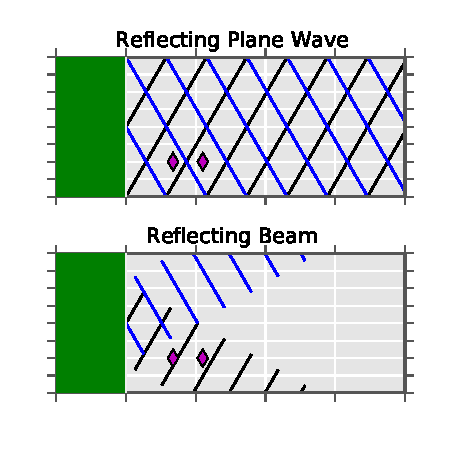
\includegraphics[width=2in]{ReflectingSketch}
    \caption{Schematic of the difficulty of quantifying reflecting fluxes in an inhomogeneous environment.  Plane waves are trivial.  Inhomogeneous incoming waves or reflections are significantly more difficult.  
      \tempS{\footnotesize /Users/jklymak/ttide/ttide15/doc//PaperPlots.ipynb ;     
        /Users/jklymak/ttide/ttide15/doc/ReflectingSketch.pdf}
     } \label{fig:ReflectingSketch} 
  \end{center}
\end{figure}

Here we run numerical simulations that are meant to represent a mode-1 internal $M_2$ tide incident on the Tasman Slope, east of Tasmania.  The simulations are only forced by the incident internal tide, and there is no local forcing, allowing the reflection signal to be isolated.  After discussing the model setup \fref{sec:Model}, we briefly consider the response this forcing has on the slope \fref{sec:Real} and compute and energy budget of the complete response.  In order to separate the physics of the reflection, we then simplify the geometry \fref{sec:Simplified}, both geometrically, and by removing parts of the topography.  This technique allows us to separate incident and reflected signals from the total response without appeal to plane wave fits.  We end with a discussion of the results (\fref{sec:Discussion}) where we note the applicability of two-dimensional reflection models and discuss the leaky slope waves evident in the simulations.  We conclude with a summary (\fref{sec:Summary}).


\section{Model setup}
\label{sec:Model}


\begin{figure*}[htbp]
  \begin{center}
    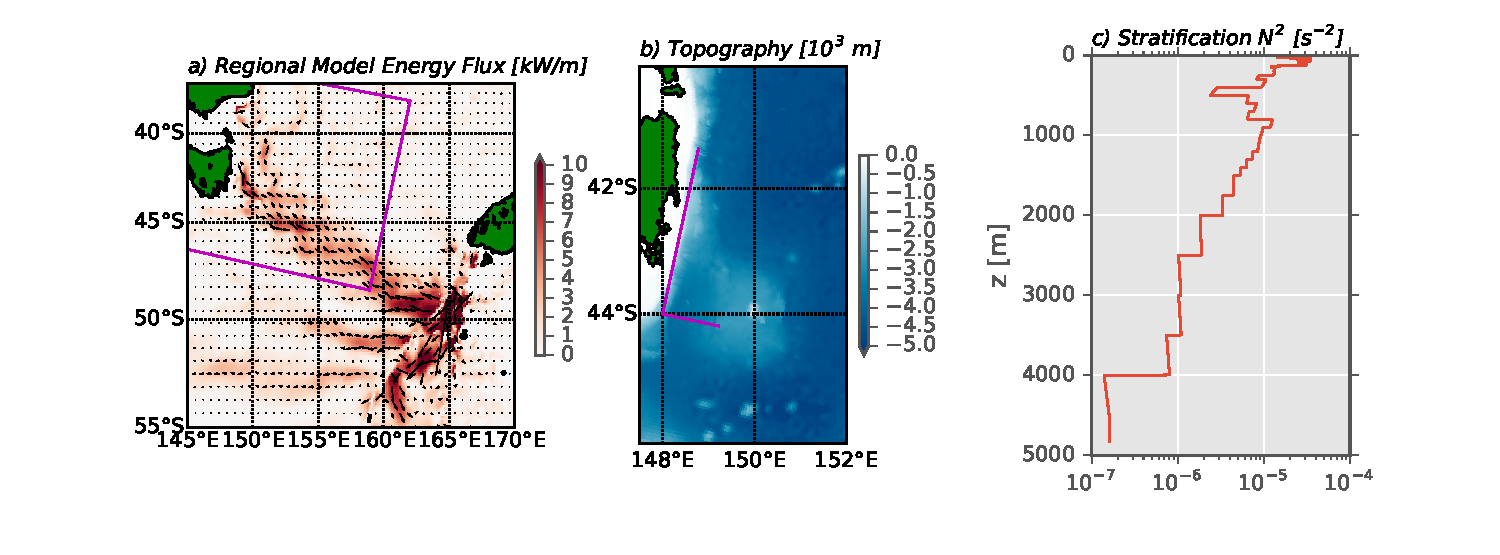
\includegraphics[width=6.5in]{./doc/LocMap.pdf}
    \caption{Location of TTide experiment: a) Energy flux in a regional numerical simulation.  Color is the absolute value of the flux, arrows it's direction.  The magenta box indicates the numerical modeling domain used in this paper.  b) Detail of the bathymetry on the Tasman slope.  The magenta lines indicate 100 km in the x-direction, and 300 km in the y direction in the modeling domain used in this paper.
      \tempS{\footnotesize /Users/jklymak/ttide/ttide15/doc//PaperPlots.ipynb ;     
        /Users/jklymak/ttide/ttide15/doc/LocMap.pdf}
      \label{fig:LocMap} }
  \end{center}
\end{figure*}

\subsection{Basics}

The numerical model used here is the MITGCM \citep{marshalletal97}, visualized using the Python scientific stack \citep{hunter07,vanderwaltetal11}. The setup is very similar to \citet{buijsmanetal14}, with the model run in hydrostatic mode, background (isotropic) diffusivities and viscosities of $10^{-5}\ \mathrm{m^2\,s^{-1}}$, and enhanced diffusivity and viscosity in regions of temporarily unstable stratification \citep{klymaklegg10}.  A second-order flux-limiting temperature advection scheme is used which results in some numerical dissipation and diffusion.  Sensitivity tests were run with weaker forcing, and the fraction of energy dissipated in the model did not change, indicating that the dissipation highlighted below is dominated by numerical dissipation due to the lack of lateral resolution (1 km) rather than explicit viscosities. Dissipation is not the main focus of this paper, and finer resolutions have been used for more focused efforts dealing with turbulence on the slope (in preparation).  These simulations are therefore the most ``linear'' that the resolution will allow.  

Topography is from a data set that combines \citet{smithsandwell97} and multibeam data from Australian surveys \citep{Whiteway09a} (\fref{fig:LocMap}b).  For this paper, we use a Cartesian co-ordinate system centered at 44 S, 148 E, with $y$ pointing 12 degrees east of geographic north (magenta lines, \fref{fig:LocMap}).  This co-ordinate system is close to cross-slope in the x-direction, and is used for conceptual convenience.  The simulations are run on a f-plane ($f=-10^{-4}\ \mathrm{s^{-1}}$).  

A 1-km lateral resolution is used along the continental slope (\fref{fig:AnalyticalForcing}a, smallest inset green box).  Resolution is expanded by 3.5\% per grid cell beyond the 1km-resolution region, to a maximum of 5 km in the second largest inset box (\fref{fig:AnalyticalForcing}a); this keeps the resolution over the Tasman Rise and the rest of the continental slope at least 5 km.  Further out, the grid spacing is again increased at 3.5\% per grid cell until a maximum grid cell size of 10 km is reached.  

Vertical resolution is approximately stretched so $dz\sim 1/N$, where $N^2(z)=-\frac{g}{\rho_0}\frac{d\rho}{dz}$ is the vertical stratification.  200 vertical grid cells are used for these simulations. The vertical stratification is from the World Ocean Atlas for the Tasman Sea just offshore of Tasmania \citep{woa13}, and is assumed laterally constant in the domain.  This precludes any mesoscale effects, which are believed to be important in this area, and are the subject of future work.



%
%$x' = m(\Phi-\Phi_o)\cos(\Theta_0)$
%
%$y' = m(\Theta-\Theta_o)$
%
%$x = x'\cos(\theta_0) + y'\sin(\theta0)$ 
%
%$y = y'\cos(\theta_0) - x'\sin(\theta0)$ 
%
%$\theta_0=12^o$
%
%? Check rotation
%
%where $m= 111.192\ \mathrm{km/degrees}$.  

\subsection{Forcing}

To simplify the generation problem we apply an analytical forcing to our model.  This is composed of two line sources at approximately the location of the Macquarie Ridge (\fref{fig:AnalyticalForcing}a).  The initial conditions and the southern and eastern boundaries of the model were set with this forcing.  The forcing is similar to that suggested by \citet{rainvilleetal10}, except instead of a single point source placed a distance $R$ from the line source, the line source is digitized as a number of discrete point sources and their response in the domain summed.  The mode-1 pressure anomaly is given by:
\begin{equation}
  p'(x,y,t)=\sum_{i=1}^{N}  a_i \exp\left(j\left(|k_t|r_i - \omega t\right)\right)
\end{equation}
where $r_i=\sqrt{\left(x-x_i\right)^2+\left(y-y_i\right)^2}$ is the distance to the source, and $|k_t|$ is the absolute value of the mode-1 wavenumber:
\begin{equation}
  k_t = \frac{\left(\omega^2-f^2\right)^{1/2}}{c_e}
\end{equation}
where $\omega$ is the frequency of the tide, $f$ is the Coriolis frequency, and $c_e$ is the eigenspeed of the vertical mode equation:
\begin{equation}
  \frac{d}{dz}\left(\frac{1}{N^2}\frac{d\psi}{dz}\right)
 + \frac{1}{c_e^2}\psi(z)=0.
\end{equation}
Here $\psi(z)$ is the eigenfucntion that sets the shape of the vertical mode, and the boundary conditions are $d\psi/dz=0$ at $z=0$ and $z=-H$, where $H$ is the water depth.  For convenience, we normalize $\psi_m(z)$ so that 
\begin{equation}
  \int_{-H}^0 \psi_m(z)\psi_n(z)\, dz = \delta_{mn}.
\end{equation}
Horizontal velocities can be linearly decomposed by these shapes, as can the pressure signal.  

To compute the wavefield, the horizontal velocity components are derived from the internal wave consistency relations: 
\begin{eqnarray}
  u(x,y,t) & = &\sum_{i=1}^{N}  \frac{k_x\omega + j k_y f}{\omega^2-f^2} \frac{p_i'}{\rho}\\
  v(x,y,t) &=& \sum_{i=1}^{N}  \frac{k_y\omega - j k_x f}{\omega^2-f^2} \frac{p_i'}{\rho} 
\end{eqnarray}
where $k_x=k_t\cos(\theta_i)$ and $k_y=k_t\sin(\theta_i)$ are calculated from the angle to  each element of the line sources $\theta_i = \arctan((y-y_i)/(x-x_i))$.  

\begin{figure*}[htbp]
  \begin{center}
    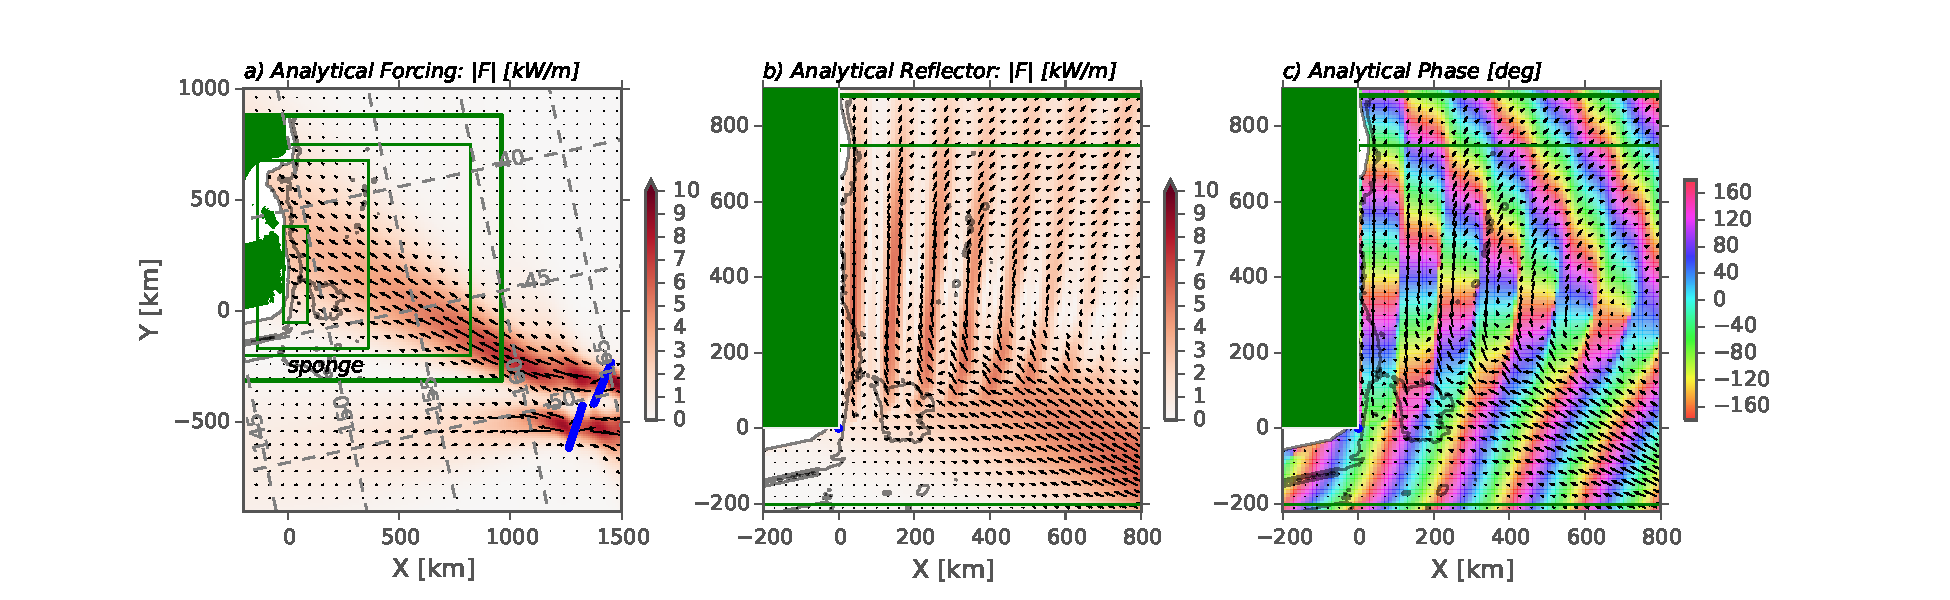
\includegraphics[width=8in]{AnalyticalForcing}
    \caption{a) Forcing used to drive the models used in this paper.  Two mode-1 internal wave sources are located to the south east (blue lines).  The model domain is rotated 12 degrees from geographic so the shelf break approximately lies along $x=0$.  Typical model domain and sponge region is indicated as green rectangles.   The 250, and 3000-m isobaths are contoured.  Arrows show the direction of the energy flux, and are scaled by its strength.  
    b) Energy flux of analytical response of energy reflecting from a wall at $x=0$, north of $y=0$.    c) Phase of reflected response. 
      \tempS{\footnotesize /Users/jklymak/ttide/doc//PaperPlots.ipynb ;     
        /Users/jklymak/ttide/doc/AnalyticalForcing.pdf}
       }\label{fig:AnalyticalForcing}
  \end{center}
\end{figure*}

The resulting incoming wavefield (\fref{fig:AnalyticalForcing}a) has a beam of energy flux that radiates northwest, and is relatively tightly focused. The interference pattern creates a null to the south and north, and a secondary beam that radiates due west.  This schematic agrees with more realistic regional tidal models (H.\ Simmons, in preparation), and the amplitude of the beam was tuned to give approximately  $2\ \mathrm{kW\,m^{-1}}$ incident at Tasmania. Note this is less than estimates from altimetry and numerical simulations, and is purposely low to keep the runs as ``linear'' as possible.  The initial condition is applied uniformly through the domain, regardless of bathymetry, so there are some start-up transients as the proper baroclinic flow develops.  

The northern and western boundaries are sponges where the velocity is slowly dropped to zero and the stratification relaxed to the initial stratification (\fref{fig:AnalyticalForcing}a, green rectangles).  Our main focus is the area from y=0 to 400 km, so the boundaries are sufficiently far that small residual reflections do not affect the response.

The ideal response off the Tasman topography would be as a plane-wave reflection from a wall at $x=0\ \mathrm{km}$ \citep[i.e.][]{johnstonetal15}.  Here we have a relatively confined beam, but we can make a start by considering the reflection the beam from a wall at $x=0\ \mathrm{km}$ for $y>0\ \mathrm{km}$ (\fref{fig:AnalyticalForcing}b,c) using the method of images with identical line sources mirrored about the y-axis, and their phase shifted by $180\ \mathrm{deg}$.  The reflection pattern that sets up is not entirely regular, but has some straight-forward features.  The incoming beam impacts the wall at approximately $30\ \mathrm{deg}$. The horizontal wavelength of an $M_2$ internal tide is $178\ \mathrm{km}$, so the standing wave in the x-direction will have a wavelength $178/\cos(30) \approx 200\ \mathrm{km}$ and in the y-direction will have a wavelength of approximately $350\ \mathrm{km}$.  These spatial scales are readily apparent in the analytical forcing despite the non-plane-wave character of the idealized forcing (\fref{fig:AnalyticalForcing}c).  Note that the standing energy flux (\fref{fig:AnalyticalForcing}b) has peaks and nulls in absolute value, with the peaks having large flux to the north. The peaks are every half cross-slope wavelength (i.e.\ 100 km).  The nulls have weak southward energy flux (though it is difficult to discern from the subsampled arrows in the plot).  

\section{Realistic model simulation}
\label{sec:Real}

The response of the forcing in the most real bathymetry motivates the more idealized experiments that follow.  From the initial forcing (\fref{fig:VelFluxReal1km03}a), a complex wavefield develops with clear scattering from the Tasman Rise, the shelf, and numerous small inhomogeneities on the sea floor (\fref{fig:VelFluxReal1km03}b--d).  Looking along slope, the phase of the velocity signal can be seen changing approximately every 200 km, and it changes approximately every 100 km offshelf similar to what we expecte from an oblique standing wave (compare \fref{fig:VelFluxReal1km03}h to \fref{fig:AnalyticalForcing}b).  However the pattern is complicated,  not lining up in the north-south direction and inhomogeneities in the energy  that are not accounted for by a simple two-wave model. 

\begin{figure*}[htbp]
  \begin{center}
    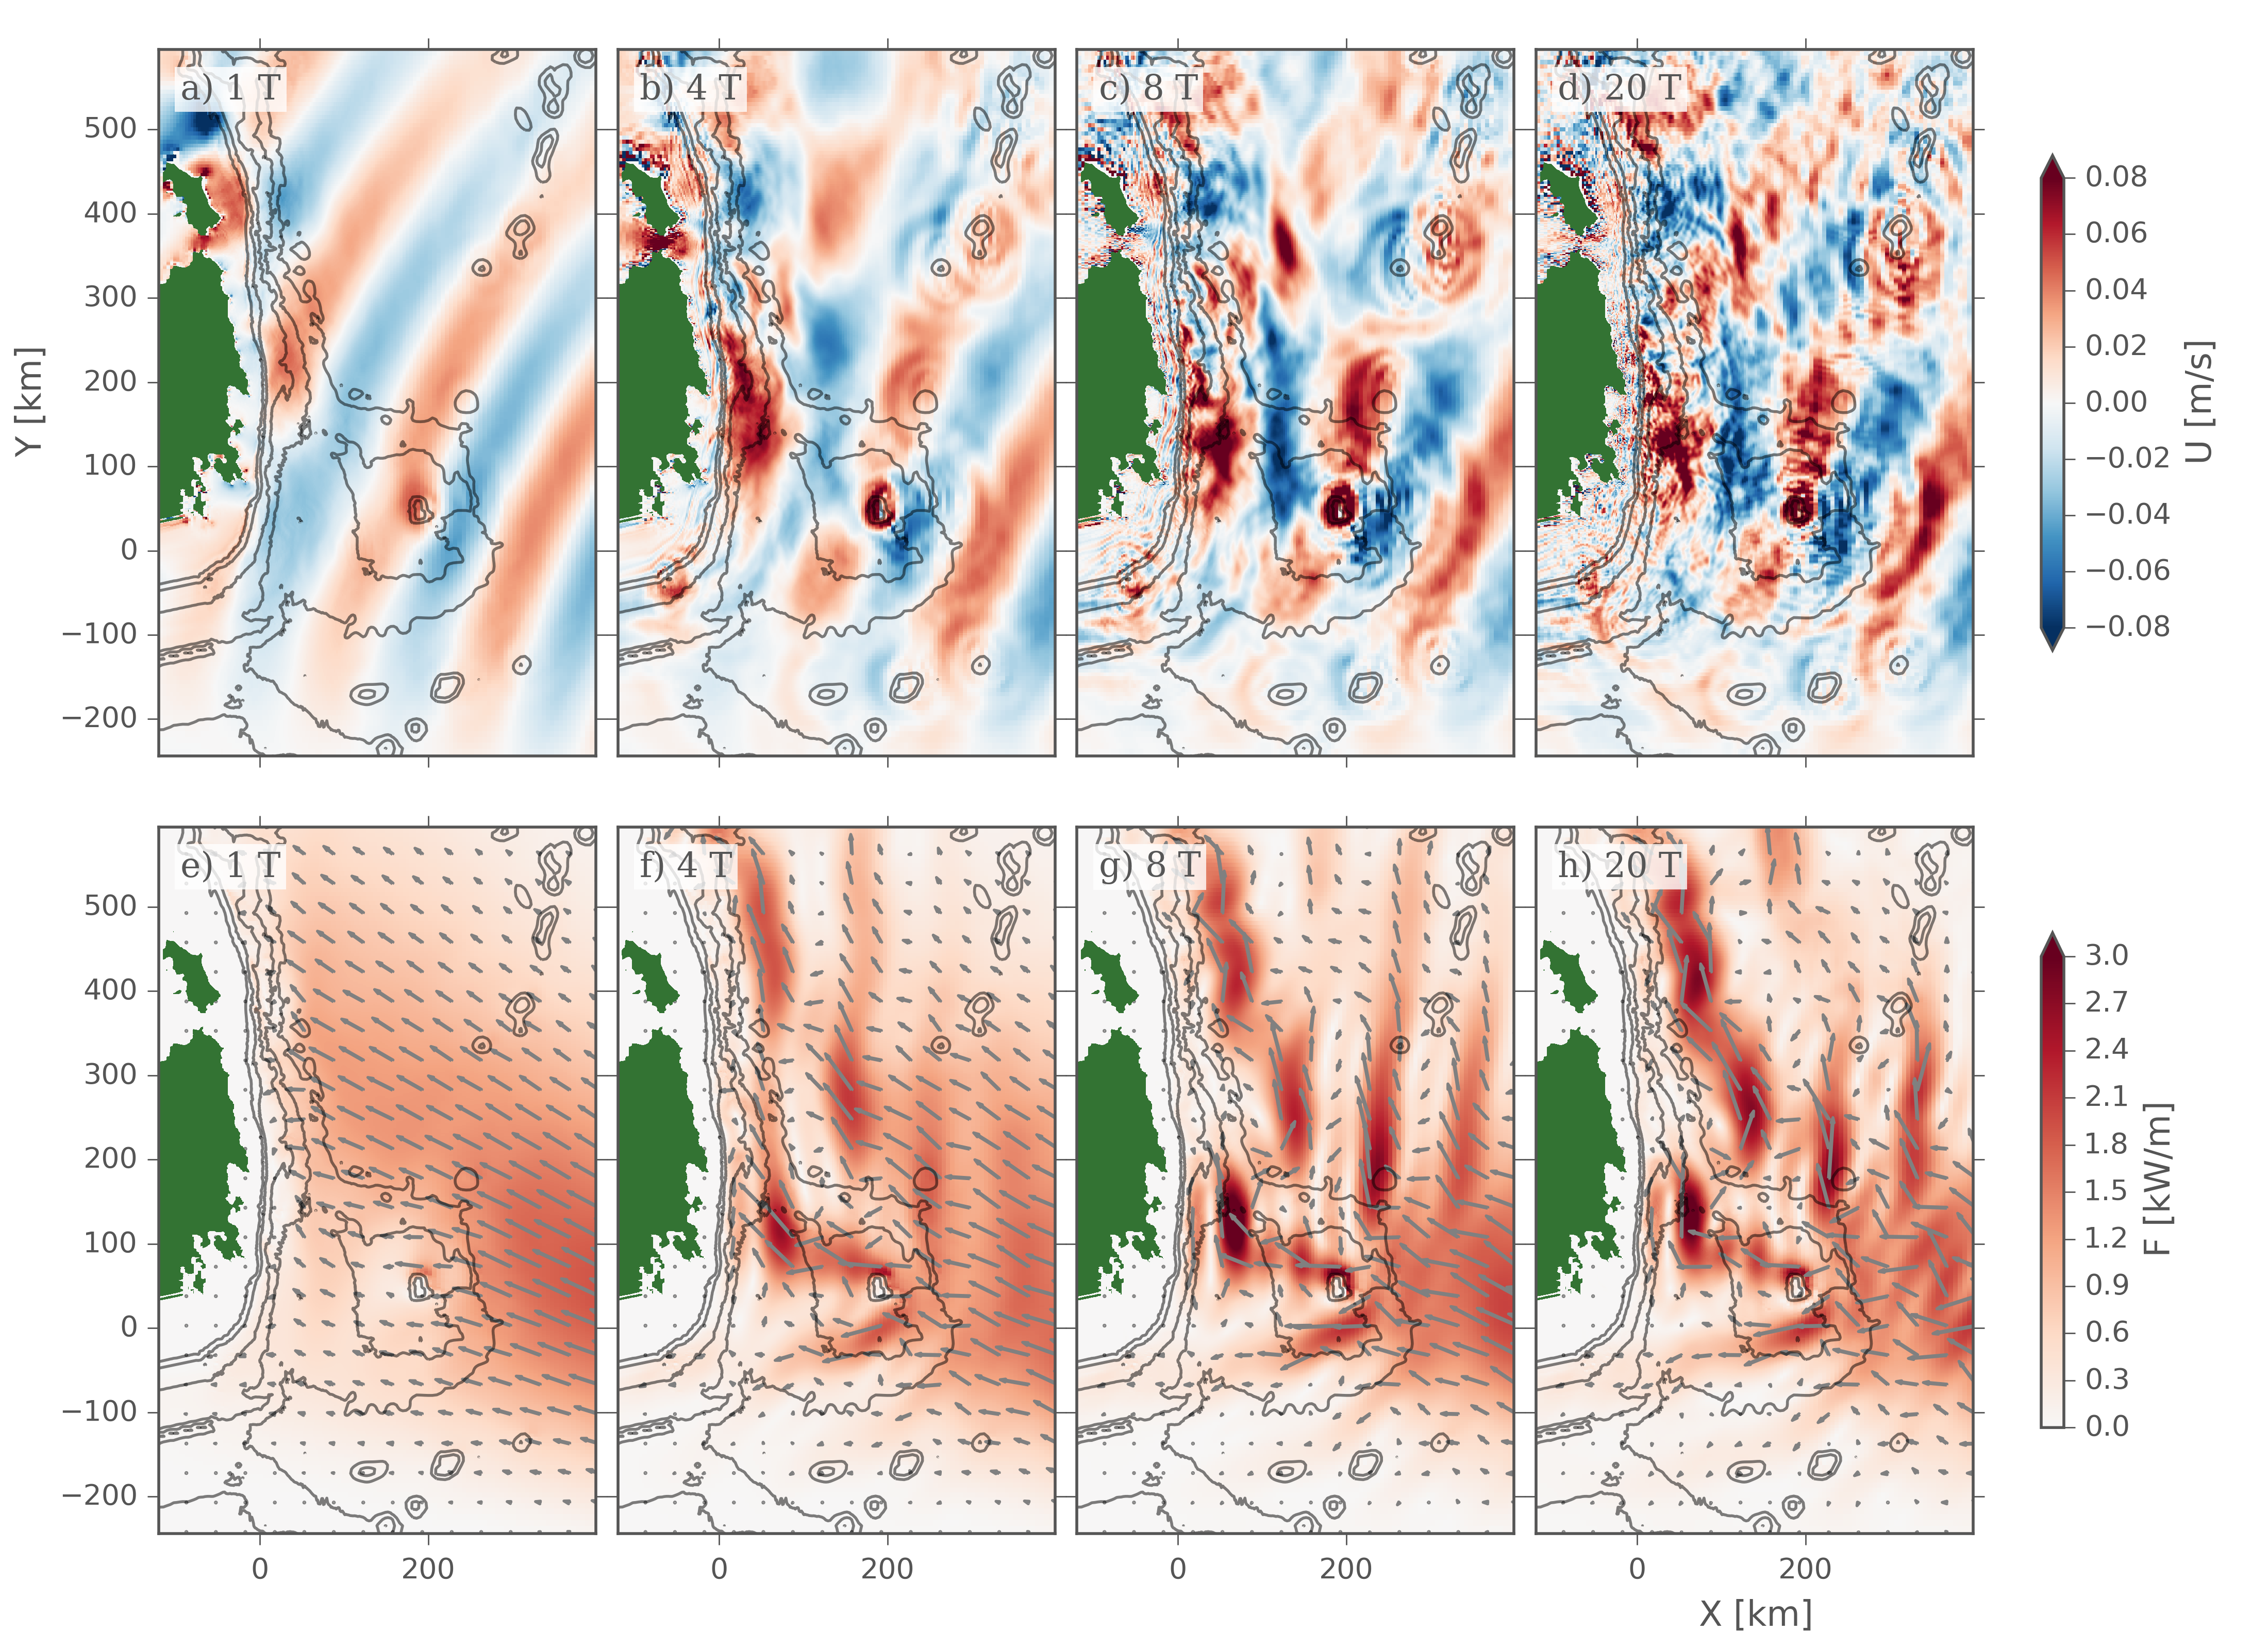
\includegraphics[width=6.6in]{VelFluxReal1km03}
    \caption{a)--d) Surface x-direction velocity for four snapshots.  a) is the initial conditions (slightly modified after a tidal cycle) and d) is the steady state. Grey contours are depths at 3000, 2000, 1000, and 250-m.  e)--h) is depth-integrated baroclinic energy flux at the same time periods, with arrows indicating direction.  
      \tempS{\footnotesize /Users/jklymak/ttide/ttide15/PaperPlots.ipynb ;     
        /Users/jklymak/ttide/doc/VelReal01.pdf}
       }\label{fig:VelFluxReal1km03}
  \end{center}
\end{figure*}

  


A time-averaged energy balance is performed online in the model using the terms outlined in \citet{kangfringer12,kang11}.  The energy balance vertically integrated can be schematized as:
\begin{equation}
  dE_{bc}/dt = -\nabla_H\cdot \mathbf{F}_{bc} + \mathrm{Conversion} - \mathrm{Dissipation}.
\end{equation}
where $E_{bc}$ is the depth-integrated baroclinic energy density, $\mathbf{F}_{bc}$ is the depth integrated energy flux, including both the pressure work term and the non-linear advection of energy (which is small in our runs).  All quantities are averaged over an $M_2$ tidal period.  ``Conversion'' is a complex term representing transfer from barotropic motions to baroclinic \citep[][eq. 5.102]{kang11} and includes the barotropic heaving of the water column, the density anomaly, and a non-linear horizontal advection term. These non-linear terms can be non-trivial in real bathymetry \citep{buijsmanetal14}.  The conversion term is positive if the barotropic tide loses energy and the baroclinic tide gains energy.  ``Dissipation'' is computed here as the residual, and includes dissipation due to explicit viscosity, numerical dissipation, and bottom drag.  

\begin{figure*}[htbp]
  \begin{center}
    \includegraphics[width=7in]{DissReal1km03cycle20}
    \caption{Energy budget over the 19th tidal cycle of 
    a) Barotropic to baroclinic conversion; b) Baroclinic energy flux convergence ($-\nabla F_{bc}$);  c) rate of change of baroclinic energy; d) residual representing the dissipation in the model $D=-\nabla \mathbf{F}_{bc}+\mathrm{Conv.} - dE/dt$.  The green box is the region for the energy time series (\fref{fig:EnergyIntegralsReal1km03}b).
      \tempS{\footnotesize /Users/jklymak/ttide/ProcessHaiseTas3d.ipynb ;     
        /Users/jklymak/ttide/doc/Diss1kmReal1km03cycle20.pdf}
       }\label{fig:DissReal1km03}
  \end{center}
\end{figure*}

Of note in the energy calculation is that the largest local term in the energy budget is an alternating pattern of barotropic-baroclinic conversion at the shelf break balanced by baroclinic flux convergences and divergences (\fref{fig:DissReal1km03}).   The importance of the barotropic-baroclinic term can also be seen by considering the x-integral of the energy budget from $x=-50\ \mathrm{km}$ to $+100\ \mathrm{km}$ (\fref{fig:EnergyIntegralsReal1km03}).  Recall that the simulations have no barotropic forcing.  This coupling is catalyzed by a start-up transient  hitting the slope with the incoming internal tide beam, and continues throughout the simulation, and is a leaky super-inertial slope wave (see \fref{sec:Discussion}).

\begin{figure}[htbp]
  \begin{center}
    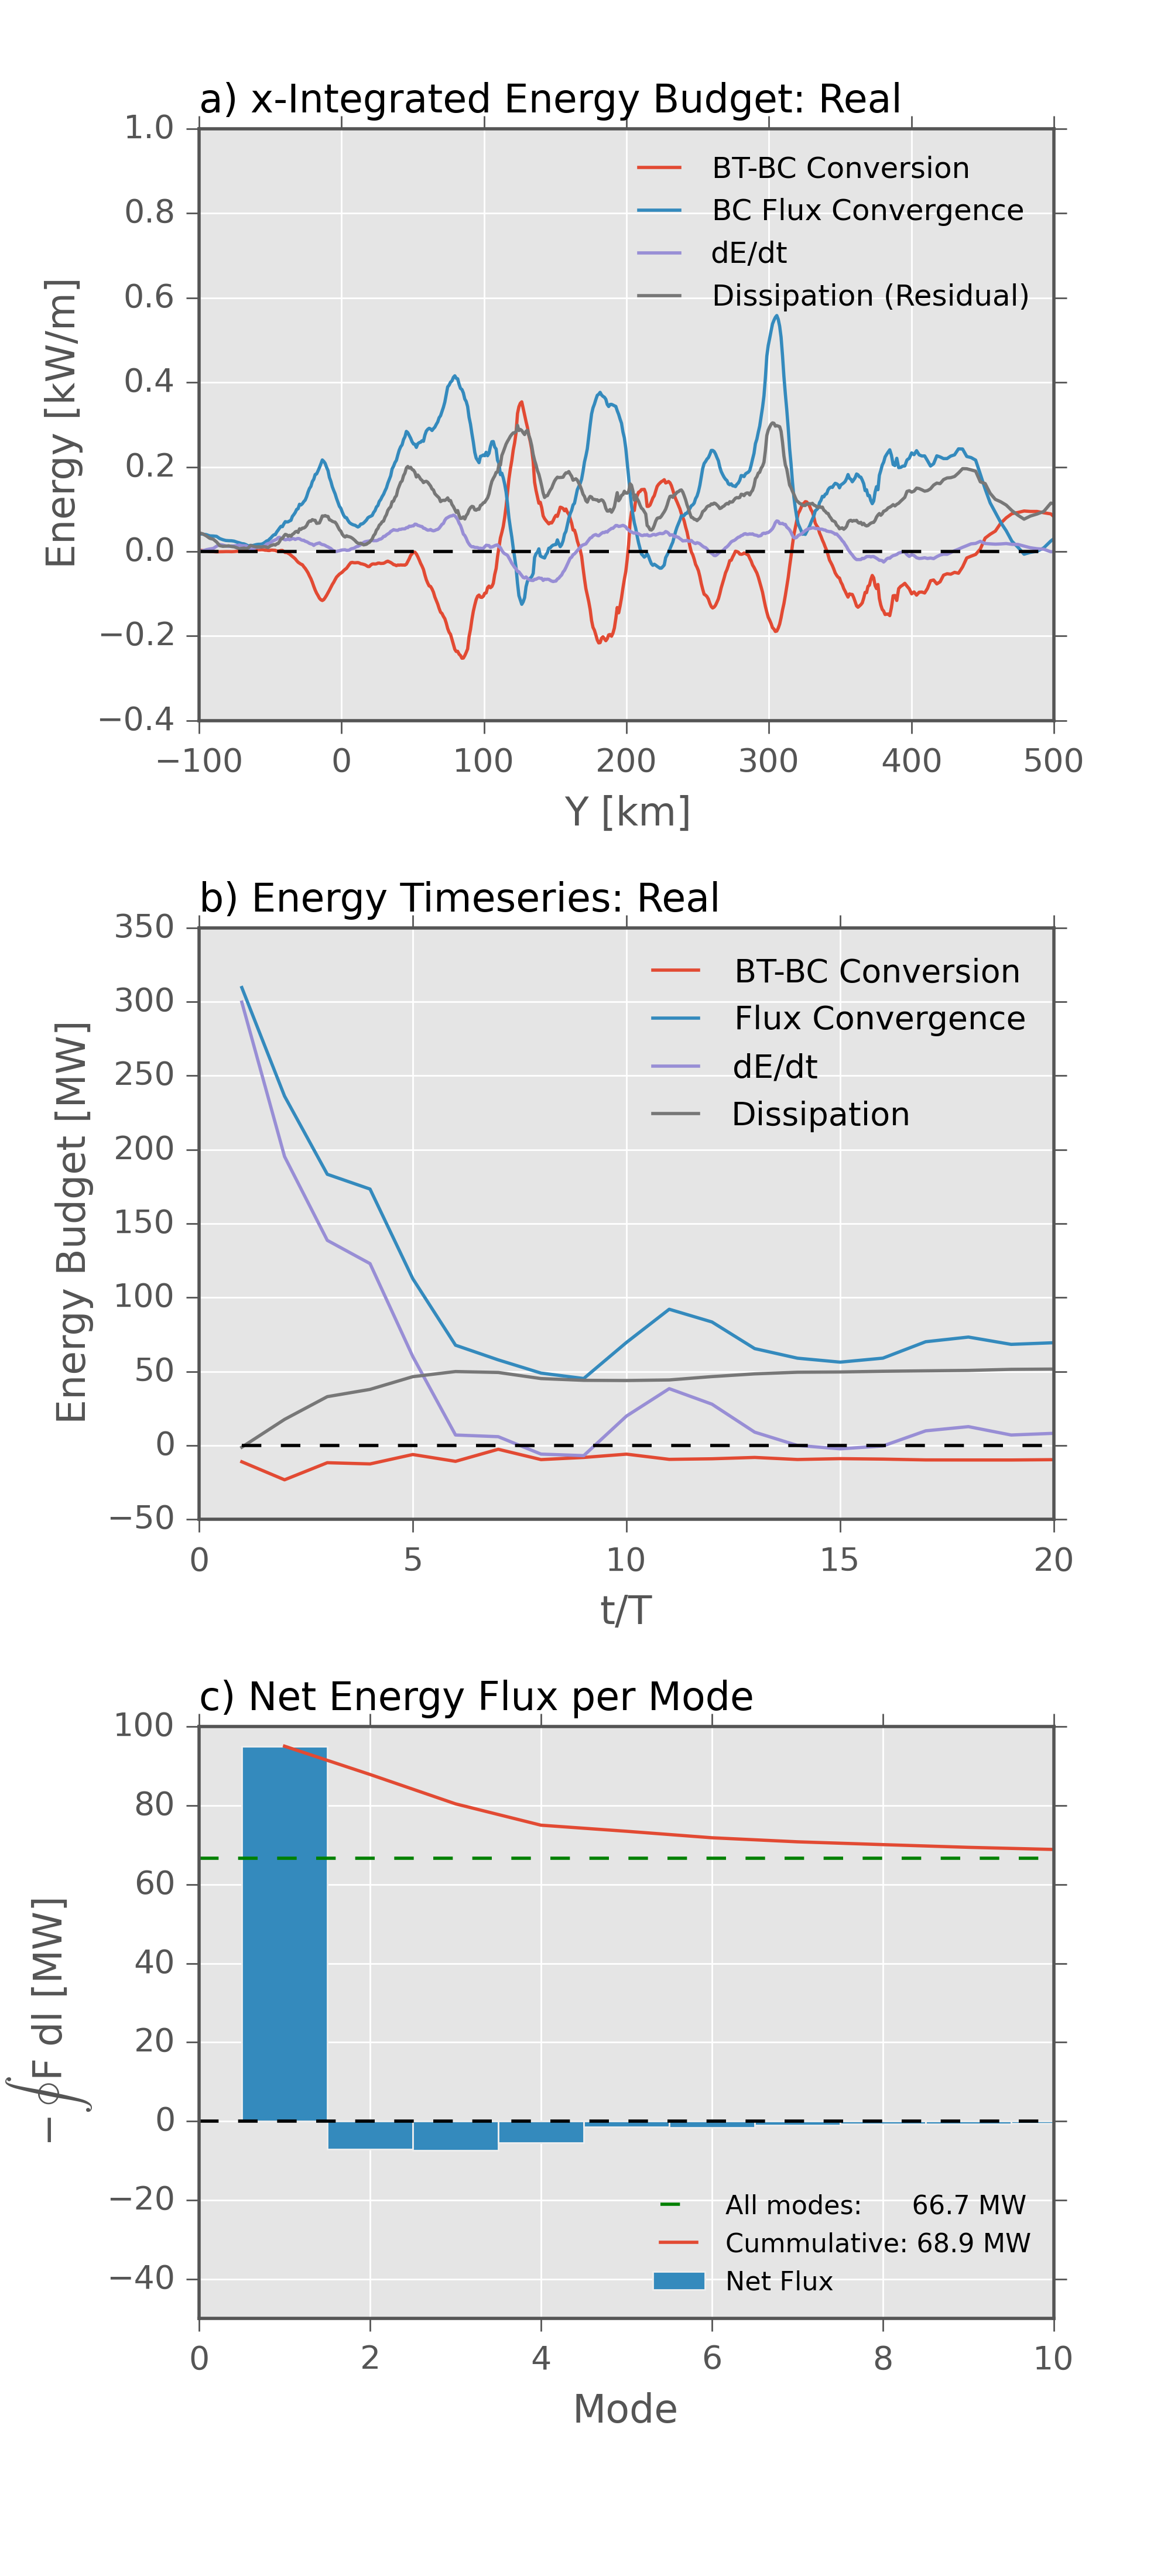
\includegraphics[width=3in]{EnergyIntegralsReal1km03}
    \caption{a) Integral in $x$ to $80\ \mathrm{km}$ offshore of the energy terms in \fref{fig:DissReal1km03} for the \mn{Real} case.  Note that the barotropic-baroclinic term (red) is of the same order as the baroclinic convergence (cyan) and the residual dissipation (gray) for most of the slope.
    b) Energy budget time series for the ``Real'' case, tidally averaged, where time is normalized by $T=12.4 h$, between $y=0$ to $y=400\ \mathrm{km}$.  There is still a small residual increase in the energy with time (purple), representing the accumulation of high-mode energy in the region. Net barotropic-baroclinc conversion (red) is small and negative, indicating a small net loss to the barotropic tide in this region. The bulk of the budget is the balance between baroclinic flux convergence (blue) and the residual ``dissipation'' (gray).
    c) Net flux in the box defined by $0<x<80\ \mathrm{km}$, and $0<y<400\ \mathrm{km}$.  Green is the value for the net flux (no modal decomposition).  Blue bars are the modal decomposition.  There is a net incoming flux in mode 1 and net reflecting fluxes in higher modes (primarily modes 2-4).
      \tempS{\footnotesize /Users/jklymak/ttide/ttide15/doc//PaperPlots.ipynb ;     
        /Users/jklymak/ttide/ttide15/doc/EnergyIntegralsReal1km03.pdf}
     } \label{fig:EnergyIntegralsReal1km03}
  \end{center}
\end{figure}

The time series of the energy terms integrated along the slope demonstrates that the barotropic-to-baroclinic term is relatively small when averaged, with a small loss of energy from the baroclinic tide to the barotropic in the integral region (\fref{fig:EnergyIntegralsReal1km03}b).  The model is largely in a steady state by tidal cycle 15, with some residual oscillations in $dE/dt$ and the flux convergence.  The large-scale baroclinic energy changes do not change the dissipation residual very much, which is relatively constant after 5 tidal cycles.  To put the 50 MW of dissipation into context, the initial energy that comes in the east and south sides of this analysis box in the initial conditions is $315\ \mathrm{MW}$, so the model is dissipating about 17\% of the incoming energy.  However, note that the dissipation is not the focus of these model runs nor of this paper. The forcing here is approximately a factor 3 lower than the real forcing, so its likely the fraction of dissipation at this site is higher if real forcing is used.  

The majority of the energy budget is in the first vertical mode (\fref{fig:EnergyIntegralsReal1km03}c).  Net fluxes in the region directly offshore of the shelf break ( $0<x<80\ \mathrm{km}$, and $0<y<400\ \mathrm{km}$) are composed of substantial mode-1 energy converging on the slope (95 MW net), and some reflected energy escaping in higher modes (28.3 MW, mostly in modes 2--4).  The 95 MW net flux is made up of the incoming and reflected mode-1 energy, and separating those terms is the subject of the next section.  There is some incoming higher-mode energy as well due to scattering from the Tasman Rise, but as we will also show below, this is minor.  The spatial pattern (not shown) of the mode conversion at the continental slope indicates hot-spots for conversion.  Modes 2 and 4 have a hotspot of conversion near $y=250\ \mathrm{km}$, and mode 3 at $y=325\ \mathrm{km}$.  

\section{Simplified geometries}
\label{sec:Simplified}

To help tease apart the effects of the Tasman Rise and the non-uniform slope, we carry out a few simplified experiments (\fref{fig:TopographicProfiles}; \fref{fig:EnergyFluxesAll}).  The \mn{Real} case is the one discussed above (\fref{fig:EnergyFluxesAll}f).  The \mn{No Topo} case has no topography at all (\fref{fig:EnergyFluxesAll}a), just the beam being forced at the south and east boundaries and (mostly) absorbed at the west and north. \mn{Rise} was run with the real bathymetry west of $x=70\ \mathrm{km}$ (\fref{fig:EnergyFluxesAll}e).  Three idealized geometries simplify the physics even more: the \mn{Shelf} case has a supercritical two-dimensional continental slope running north from $y=0\ \mathrm{km}$(\fref{fig:EnergyFluxesAll}d).  \mn{Round Rise} is a 1700-m tall cylinder-shaped bump with radius of 50 km centered at approximately the same location as the Tasman Rise, with no shelf to the west (\fref{fig:EnergyFluxesAll}b).  The simplified slope and the rise are both used in the \mn{Shelf/Rise} case (\fref{fig:EnergyFluxesAll}c).  

\begin{figure}[htbp]
  \begin{center}
    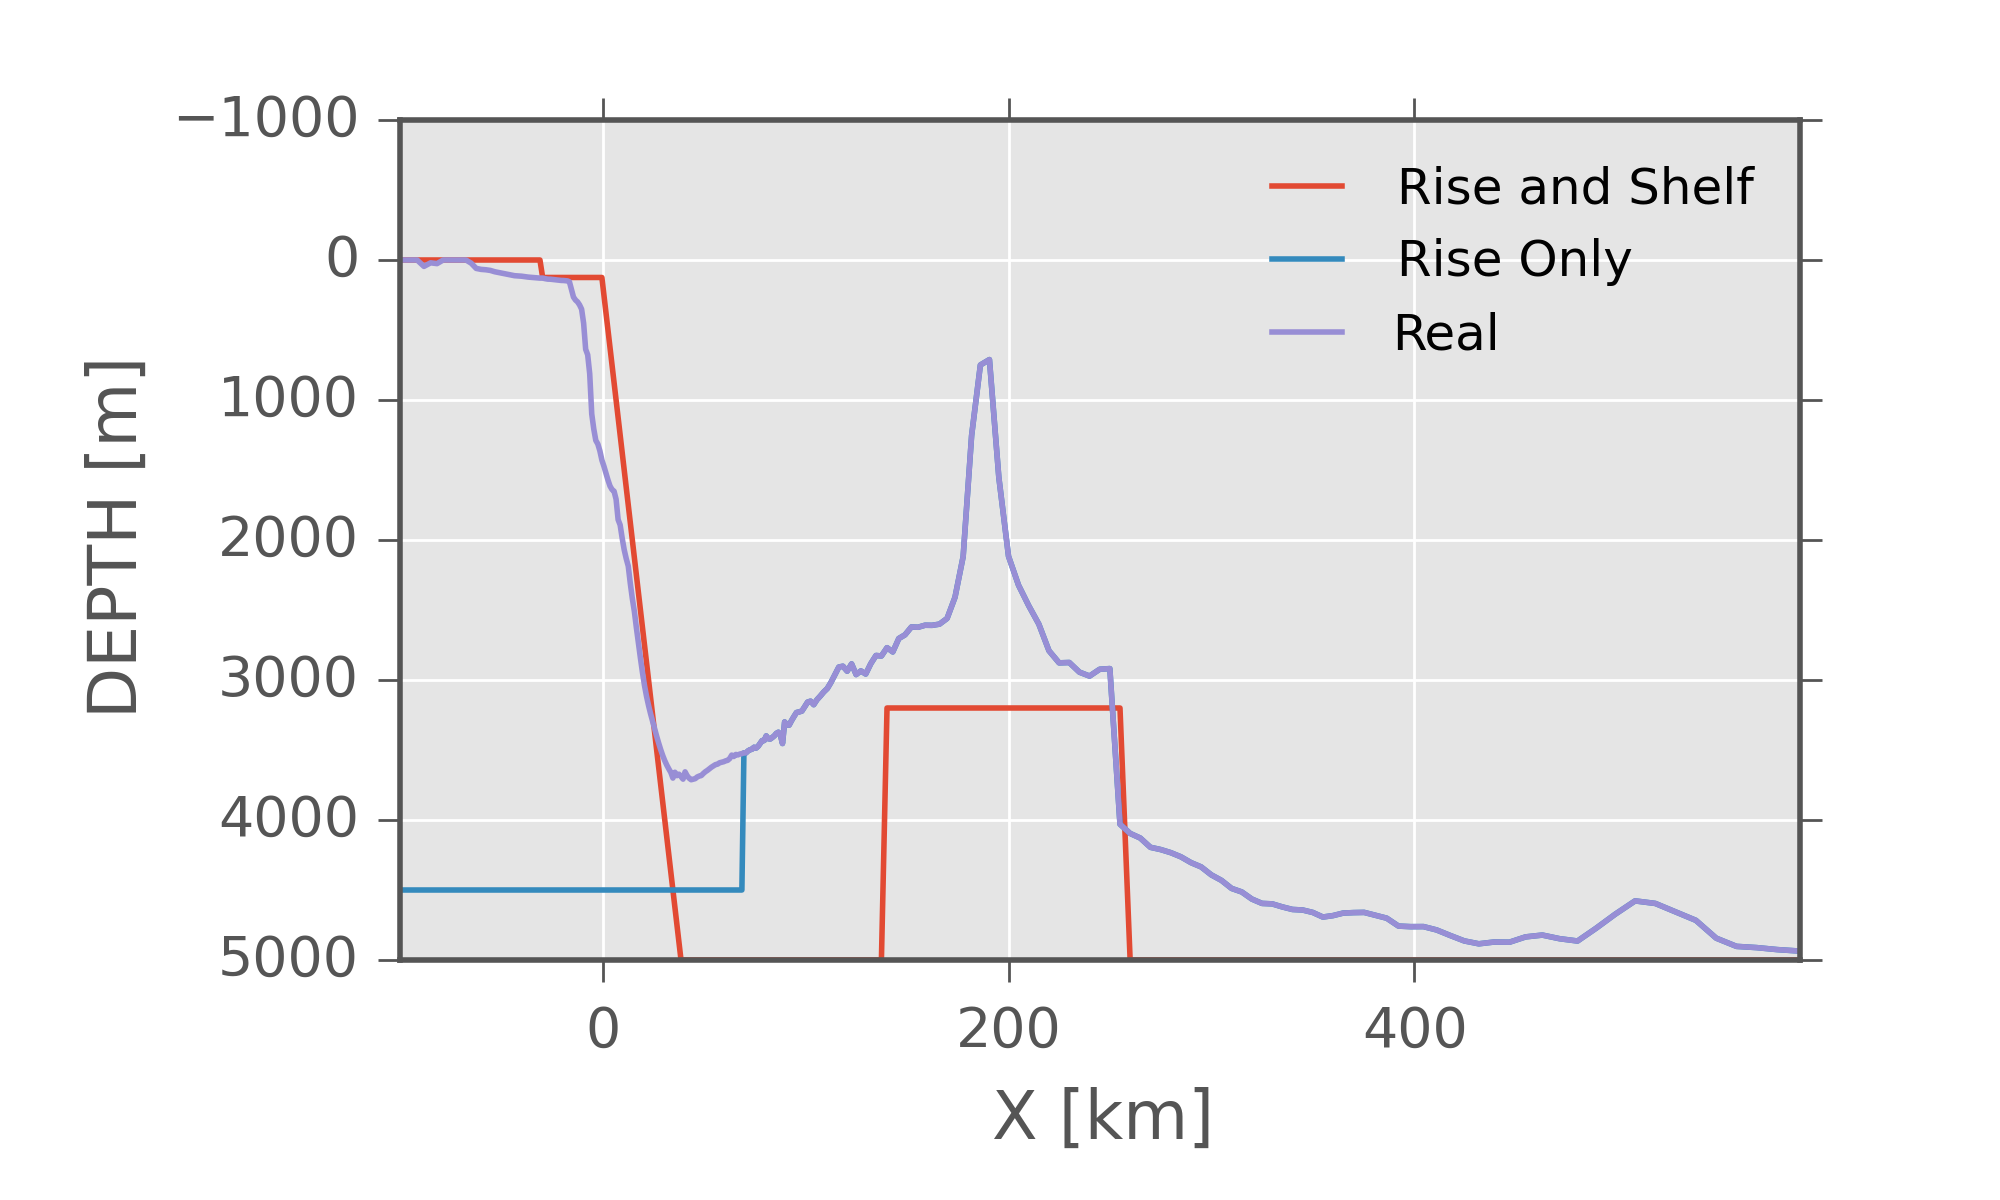
\includegraphics[width=3in]{TopographicProfiles}
    \caption{Cross sections of topographies from $y=50\ \mathrm{km}$.
      \tempS{\footnotesize /Users/jklymak/ttide/ProcessHaiseTas3d.ipynb ;     
        /Users/jklymak/ttide/doc/TopographicProfiles.pdf}
       }\label{fig:TopographicProfiles}
  \end{center}
\end{figure}

\begin{figure*}[htbp]
  \begin{center}
    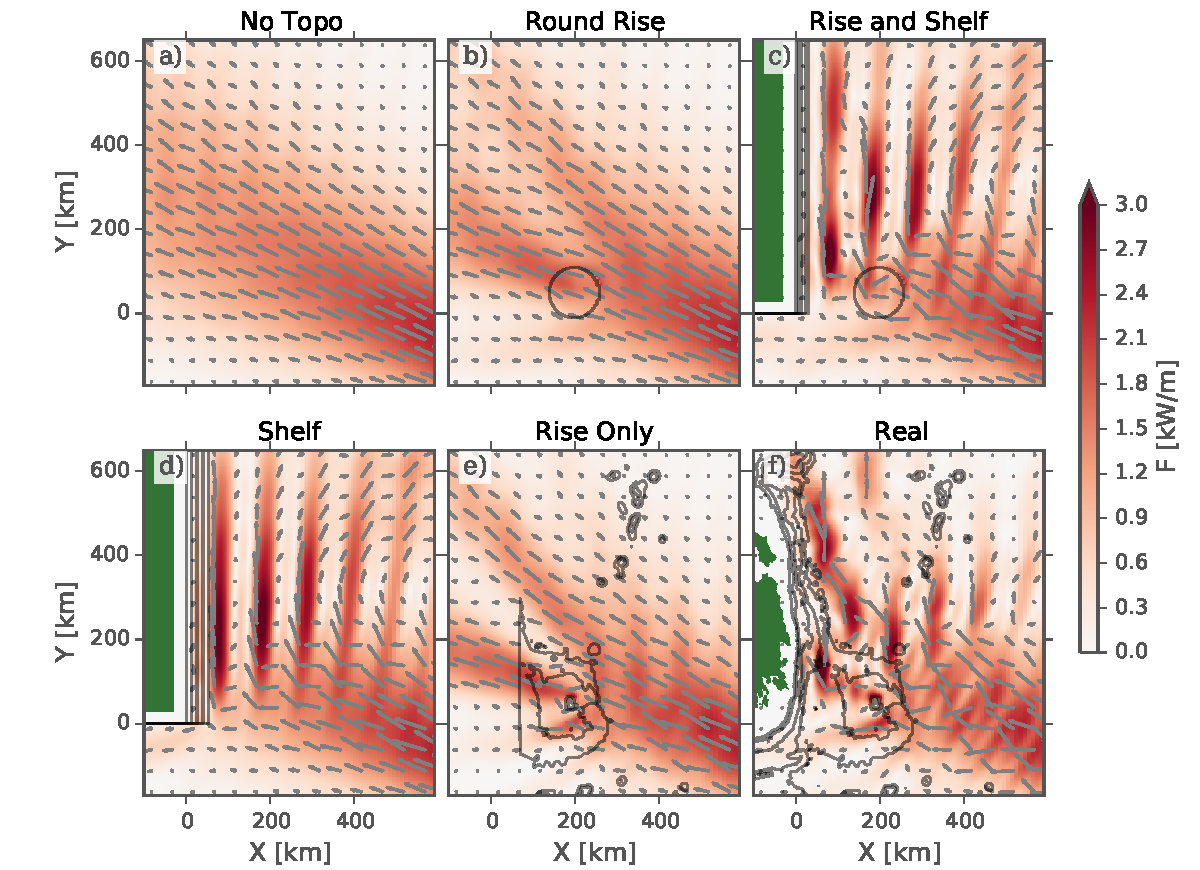
\includegraphics[width=6in]{EnergyFluxesAll}
    \caption{Energy flux for six geometries at tidal cycle 20.  Grey depth contours are -3000, -2000, -1000 and -250 m.  Arows indicate the direction of energy flux.  See \fref{fig:TopographicProfiles} for bathymetry cross sections at $y=50\ \mathrm{km}$.  
      \tempS{\footnotesize /Users/jklymak/ttide/ttide15/doc//PaperPlots.ipynb ;     
        /Users/jklymak/ttide/ttide15/doc/CompareNoTopoRiseRealFlux.pdf}
       }\label{fig:EnergyFluxesAll}
  \end{center}
\end{figure*}


\subsection{Shelf-only configuration}

The simplest topography is the \mn{Shelf} configuration (\fref{fig:EnergyFluxesAll}d).  Here we have a response that is quite similar to the analytical response calculated above (\fref{fig:AnalyticalForcing}b).  The only difference between these two cases is the narrow shelf west of $x=0\ \mathrm{km}$ and the slight slope to the continental slope.  The interference pattern between the incoming wave and the reflected wave is clear in this plot, with the same characteristic length scales as above, and a slight bending of the response due to the radial spreading of the beam.  

The goal of this paper is to determine the amount of reflectivity of the continental slope.  This is a hard number to determine in a complicated geometry, and naturally depends on the region of integration.   For the \mn{Shelf} configuration the situation is relatively simple, and we use it to illustrate the numerical technique used below.  The signal in the full simulation is assumed to consist of an ``incoming'' signal and a reflected signal, so we can decompose the east-west velocity amplitude of the first vertical mode (for example) as:
\begin{eqnarray}
  u_{1}^{t}(x,y) &= &u_{1}^{i}+u_{1}^{r}\\
  v_{1}^{t}(x,y) &= &v_{1}^{i}+v_{1}^{r}\\
  p_{1}^{t}(x,y) &= &p_{1}^{i}+p_{1}^{r}
\end{eqnarray}
where $u_{1}^t$ is the  complex amplitude of the $\mathrm{M_2}$, mode-1 east-west velocity of the simulation with the reflection, $u_{1}^i$ of the incoming signal, and $u_{1}^r$ of the reflected signal.  We assume for this example that the incoming signal $u_{1}^i$ is given by the \mn{No Topo} simulation, and $u_{1}^t$ is from the \mn{Shelf} simulation.  The reflected signal $u_1^r$ is simply the difference of these two.  This method has been used by \citet{halletal13} for a two dimensional flow.  Here it is an absolute necessity because of the complicated three-dimensional topography.  

In order to compute and energy budget, we consider that the energy fluxes are calculated from the decomposed signals as:
\begin{eqnarray}
  F_{u1}^t & = & u_1^t p_1^t \\
  &= & \overbrace{u_1^ip_1^i}^{Incoming} + \overbrace{u_1^rp_1^r}^{Reflected} + 
  \overbrace{u_1^ip_1^r + u_1^rp_1^i}^{Cross\ Terms} \\
  F_{v1}^t & = & v_1^t p_1^t \\
  &= & \overbrace{v_1^ip_1^i}^{Incoming} + \overbrace{v_1^rp_1^r}^{Reflected} + 
  \overbrace{v_1^ip_1^r + v_1^rp_1^i}^{Cross\ Terms} 
\end{eqnarray}
The cross terms are not negligible for any realistic forcing, and indeed give rise to the interference patterns seen above \citep{nashetal04a,martinietal07}. 

The ``total'' response (\fref{fig:ShelfResponseMode1}d) consists of the incoming response (\fref{fig:ShelfResponseMode1}a), and the ``reflected'' signal (\fref{fig:ShelfResponseMode1}b), and substantial cross-terms (\fref{fig:ShelfResponseMode1}c).  The cross terms are mostly perpendicular to the direction of reflection (i.e. parallel to the slope) and alternately flux energy to the north and south every half cross-slope wavelength.  Combined, these three components give the ``total'' flux with net fluxes to the north in alternating peaks every full offslope wavelength.  

The reflected response (\fref{fig:ShelfResponseMode1}b) shows approximately what we would expect with energy being radiated to the north-east.  There is some concentration of this energy at $y\approx \mathrm{75 km}$, and  $y\approx\ \mathrm{225 km}$ because of coupling with a partially trapped slope wave.  This coupling causes a redistribution of the reflected energy, focusing it approximately every along-slope wavelength of the slope wave (we show in \fref{sec:Discussion} that this wavelength changes as the slope geometry changes).  

Performing this analysis for the lowest 10 modes, we arrive at an energy budget for the slope in the green box in the figures ($0<y<400\ \mathrm{km}$, and $x<80\ \mathrm{km}$; \fref{fig:ShelfResponseMode1}, inset budgets).   Note that we assume the flux through $x=0$ is zero.   With this calculation, we see that $408\ \mathrm{MW}$ is incident on the slope in mode-1.  There is also a net flux  of $50\ \mathrm{MW}$ into this region from the cross terms.  This is a redistribution of energy from north of our box into the box.  There is a net convergence of this cross-term energy because there is dissipation in the box; in a purely inviscid solution this term should balance to zero over a closed box.  If we extend the integration further north, the cross-term flux drops to zero.  

Most of the incoming energy reflects back out of the box (\fref{fig:ShelfResponseMode1}b), with the bulk remaining in mode 1, and  some scattering to higher modes.  This scattered energy radiates to the north east (not shown).  The mode-1 reflection is affected by the slope wave that transfers energy to and from the barotropic tide along the slope, resulting in nulls and peaks in the mode-1 reflection.  

\begin{figure*}[htbp]
  \begin{center}
    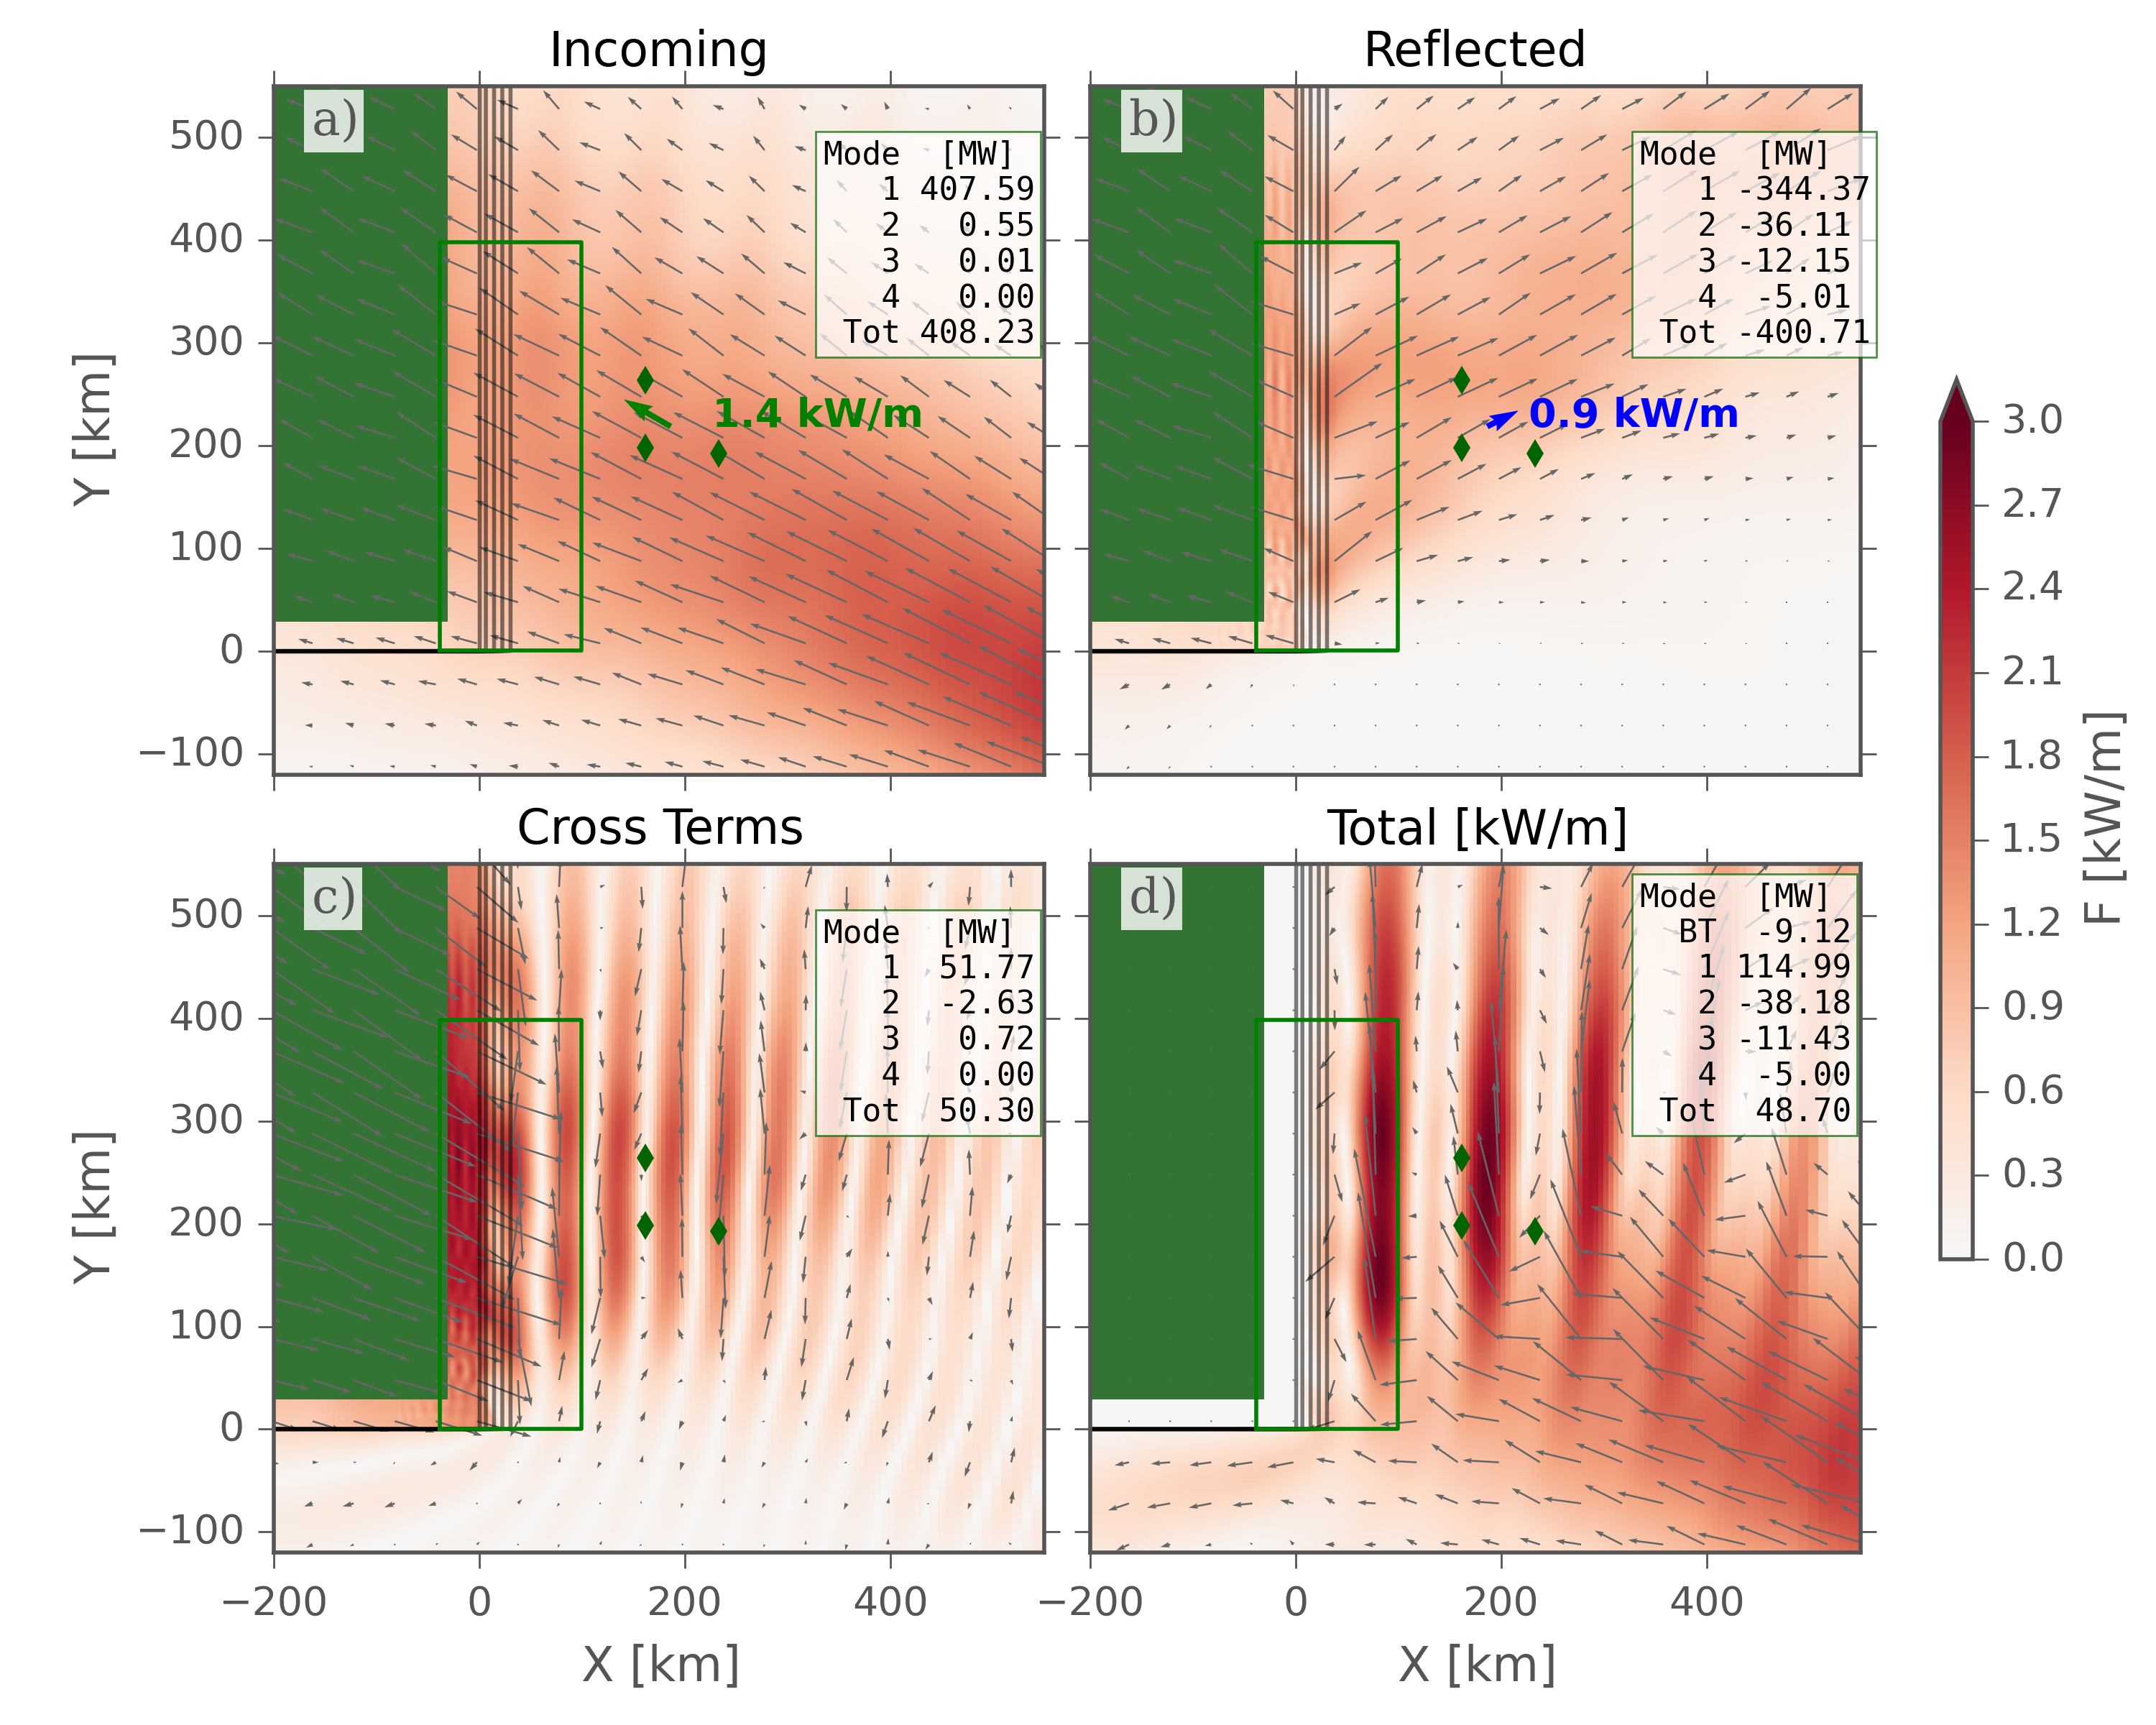
\includegraphics[width=5.5in]{ShelfResponseMode1}
    \caption{Mode-1 decomposition of energy fluxes for the \mn{Shelf} experiment.  a) Incoming energy flux calculated from the \mn{No Topo} simulation (\fref{fig:EnergyFluxesAll}a).  Note that the shelf bathymetry is contoured on this plot (grey lines, and green ``land''), but this bathymetry was not part of this simulation.  The green line demarks the region the energy budget in the inset was integrated over.  The green diamonds are the location of a synthetic mooring, and the arrow indicates the estimated incoming flux from a plane wave fit over the three moorings of the ``Total'' simulation (see text).  b) Reflected energy flux calculated from the difference between the velocities and displacements of the Total simulation (panel d) and the ``Incoming'' (panel a).  Blue arrow is the outgoing flux from a plane wave fit over the mooring array from the ``Total'' simulation.  c) Energy flux cross terms between the incoming and outgoing waves.  d) Total simulation from the \mn{Shelf} case (\fref{fig:EnergyFluxesAll}d)
      \tempS{\footnotesize /Users/jklymak/ttide/ProcessHaiseTas3d.ipynb ;     
        /Users/jklymak/ttide/doc/RiseResponseMode1.pdf}
      }\label{fig:ShelfResponseMode1} 
  \end{center}
\end{figure*}

%\begin{table}[t]
%\caption{Energy budget for the \mn{Shelf} case (all values in MW).  Budget is integrated along the east, south and north faces from $y=0$ to $400\ \mathrm{km}$ at $x=80\ \mathrm{km}$.} \label{tab:EnergyBudgShelf1km03}
%\begin{center}
%\begin{tabular}{c rrrr}
%\hline\hline
%Mode& Incoming & Reflected & Cross terms & Total\\\hline
%1 & 407.59 & -344.37 & 51.77 & 114.99\\ 
%2 & 0.55 & -36.11 & -2.63 & -38.18\\ 
%3 & 0.01 & -12.15 & 0.72 & -11.43\\ 
%4 & 0.00 & -5.01 & 0.00 & -5.00\\ \hline 
%Total & 408.23 & -400.71 & 50.30 & 57.82\\ \hline 
%\end{tabular}
%\end{center}
%\end{table}


\subsection{Tasman Rise only}

The Tasman Rise has a profound effect on the energy that impacts the continental slope (\fref{fig:EnergyFluxesAll}e and f).  The incoming beam is almost 500 km wide at $x=0$ if there is no Tasman Rise, but breaks into three narrower beams when there is a Tasman Rise (\fref{fig:EnergyFluxesAll}e).  Upstream of the rise, the effect is somewhat less energy propagating westward, with an  interference pattern towards the east indicating some back reflection.  


%\begin{figure}[htbp]
%  \begin{center}
%    \includegraphics[width=3in]{Flux0kmTasRise}
%    \includegraphics[width=3in]{Flux300kmTasRise}
%    \caption{Energy flux across $x=0\ \mathrm{km}$ and $x=300 \ \mathrm{km}$ showing the effect of the Tasman Rise.  
%      \tempS{\footnotesize /Users/jklymak/ttide/ProcessHaiseTas3d.ipynb ;     
%        /Users/jklymak/ttide/doc/Flux0kmTasRise.pdf}
%      \label{fig:Flux0kmTasRise} }
%  \end{center}
%\end{figure}

This pattern can be explained in terms of diffraction of the internal tide beam from a deep obstacle \citep[i.e.][]{johnstonetal03}.  There is a down-wave concentration of energy along the seamount's axis, a null, and sidelobes to the north and south.  In this case, the incident beam is of comparable size to the obstacle, leading to an asymmetry, and a stronger lobe to the north than south.  

Most of the response due to the Tasman Rise can be modeled simply as a cylindrical obstacle in the beam (\fref{fig:EnergyFluxesAll}b and c).  Here our obstacle is 1800 m high in 5000 m of water, and has a radius of 50 km (\fref{fig:TopographicProfiles}).  This captures most of the features of the actual Tasman Rise, despite not having a shallow spire in the center and being slightly smaller than the real Rise.  The differences make the simplified response have weaker nulls and the whole response is directed a bit further north than the real Rise.  Adding the shelf (\fref{fig:EnergyFluxesAll}c) yields a response that bears substantial similarity to the \mn{Real} forcing case.  

Decomposing into an incoming and reflected signal (\fref{fig:RiseShelfResponseMode1}) demonstrates the effect of the Tasman Rise on the response.  Less energy is incident on the control volume, largely because the diffraction redirects some of that energy to the north of $y=400\ \mathrm{km}$.  There is a strong reflection of energy where the main diffraction lobe reflects from the slope (\fref{fig:RiseShelfResponseMode1}b), and a smaller maximum just to the north ($y=250\ \mathrm{km}$) due to the along-slope wave that is strummed.  There is a reflection further north where the northern lobe of the diffraction pattern reflects.  

The incoming energy has some more high-mode content due to scattering at the cylindrical rise (\fref{fig:RiseShelfResponseMode1}a), though it is still 95\% mode-1.  The reflection is almost 80\% mode-1, with some scattering to higher modes.   The net flux shows approximately 15\% of the incoming energy is dissipated at the shelf.  


\begin{figure*}[htbp]
  \begin{center}
    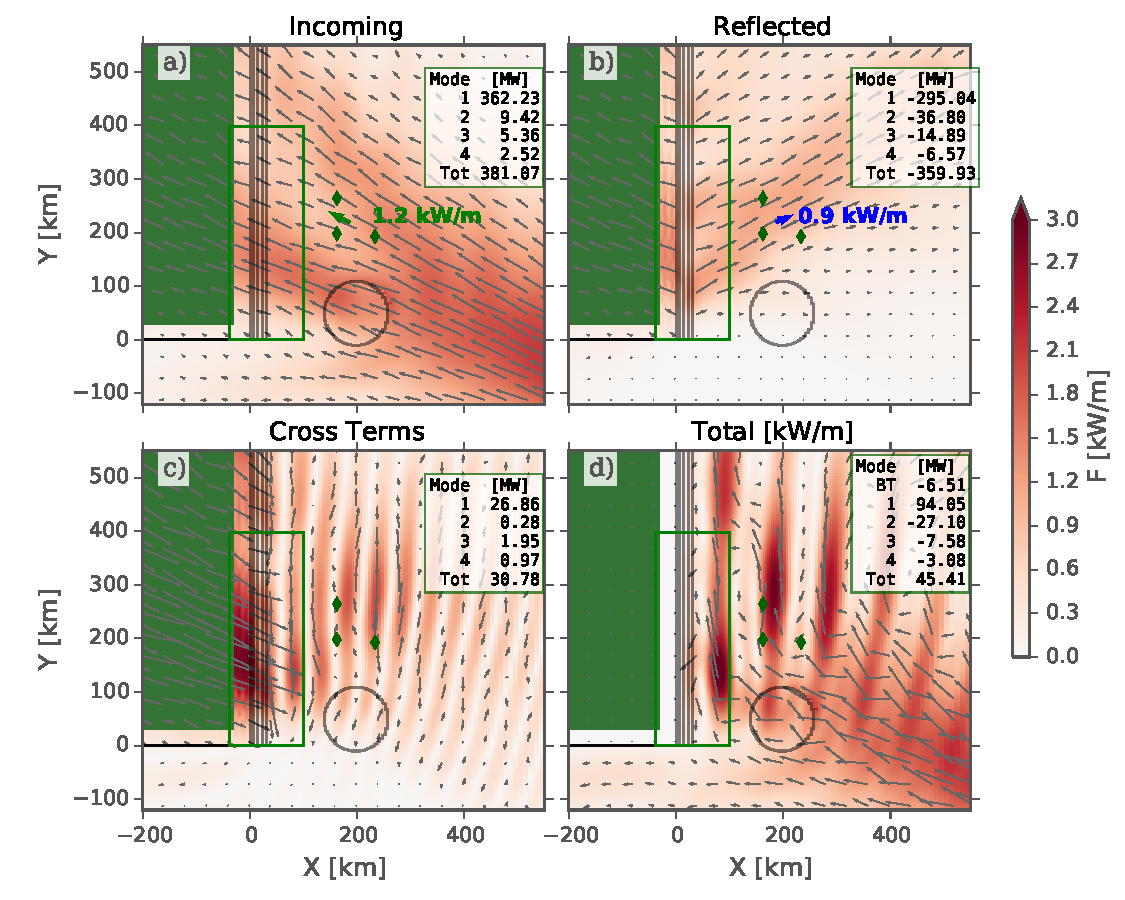
\includegraphics[width=5.5in]{RiseShelfResponseMode1}
    \caption{Energy partition as in \fref{fig:ShelfResponseMode1}, taking the \mn{Round Rise} simulation as the incoming wave, and \mn{Shelf/Rise} simulation as the total wavefield.
      \tempS{\footnotesize /Users/jklymak/ttide/ttide15/doc//ProcessHaiseTas3d.ipynb ;     
        /Users/jklymak/ttide/ttide15/doc/RiseShelfResponseMode1.pdf}
     }\label{fig:RiseShelfResponseMode1}
  \end{center}
\end{figure*}



%\begin{table}[t]
%\caption{Energy budget for the \mn{Rise-Shelf} case (all values in MW).  Budget is integrated along the east, south and north faces from $y=0$ to $400\ \mathrm{km}$ at $x=80\ \mathrm{km}$.} \label{tab:EnergyBudgRiseShelf1km04}
%\begin{center}
%\begin{tabular}{c rrrr}
%\hline\hline
%Mode& Incoming & Reflected & Cross terms & Total\\\hline
%1 & 362.23 & -295.04 & 26.86 & 94.05\\ 
%2 & 9.42 & -36.80 & 0.28 & -27.10\\ 
%3 & 5.36 & -14.89 & 1.95 & -7.58\\ 
%4 & 2.52 & -6.57 & 0.97 & -3.08\\ \hline 
%Total & 381.07 & -359.93 & 30.78 & 51.92\\\hline
%\end{tabular}
%\end{center}
%\end{table}
%

%
%\begin{figure*}[htbp]
%  \begin{center}
%    \includegraphics[width=6in]{RiseResponseMode1}
%    \caption{Energy decomposition based on taking the \mn{No Topo} case as the incoming wave, and \mn{Rise} as the total wavefield and looking at the energy flux of the difference between their waves (reflected wave field) and the energy flux associated with the cross terms between.  
%      \tempS{\footnotesize /Users/jklymak/ttide/ProcessHaiseTas3d.ipynb ;     
%        /Users/jklymak/ttide/doc/RiseResponseMode.pdf}
%      \label{fig:RiseResponseMode1} }
%  \end{center}
%\end{figure*}
\subsection{Real Case}

The \mn{Real} forcing is similar, if more complex (\fref{fig:RealResponseMode1}).  The simulation using the bathymetry in the \mn{Rise Only} case (\fref{fig:EnergyFluxesAll}e)  is used as the ``Incoming'' energy flux, and the \mn{Real}  (\fref{fig:EnergyFluxesAll}f)  case is the ``Total''.  Compared to the cylindrical rise,  the real Tasman Rise creates a sharper diffraction pattern, and more back reflection.  However, the \mn{Real} simulation has many of the same features as the \mn{Shelf/Rise} simulation (\fref{fig:EnergyFluxesAll}c).  

Slightly less incoming energy passes into the control volume (\fref{fig:RealResponseMode1}a) because the diffraction by the real Tasman Rise is sharper than the cylindrical rise.  As for the cylindrical rise case, there is some incoming higher mode energy due to forward scattering, though again over 95\% is mode-1.  Reflection is concentrated near $y=125\ \mathrm{km}$ and $y=450\ \mathrm{km}$, associated with the diffraction nodes, with about 85\% in mode 1 (\fref{fig:RealResponseMode1}b).  Dissipation is less than 25\% of the incoming energy (\fref{fig:RealResponseMode1}d).

\begin{figure*}[htbp]
  \begin{center}
    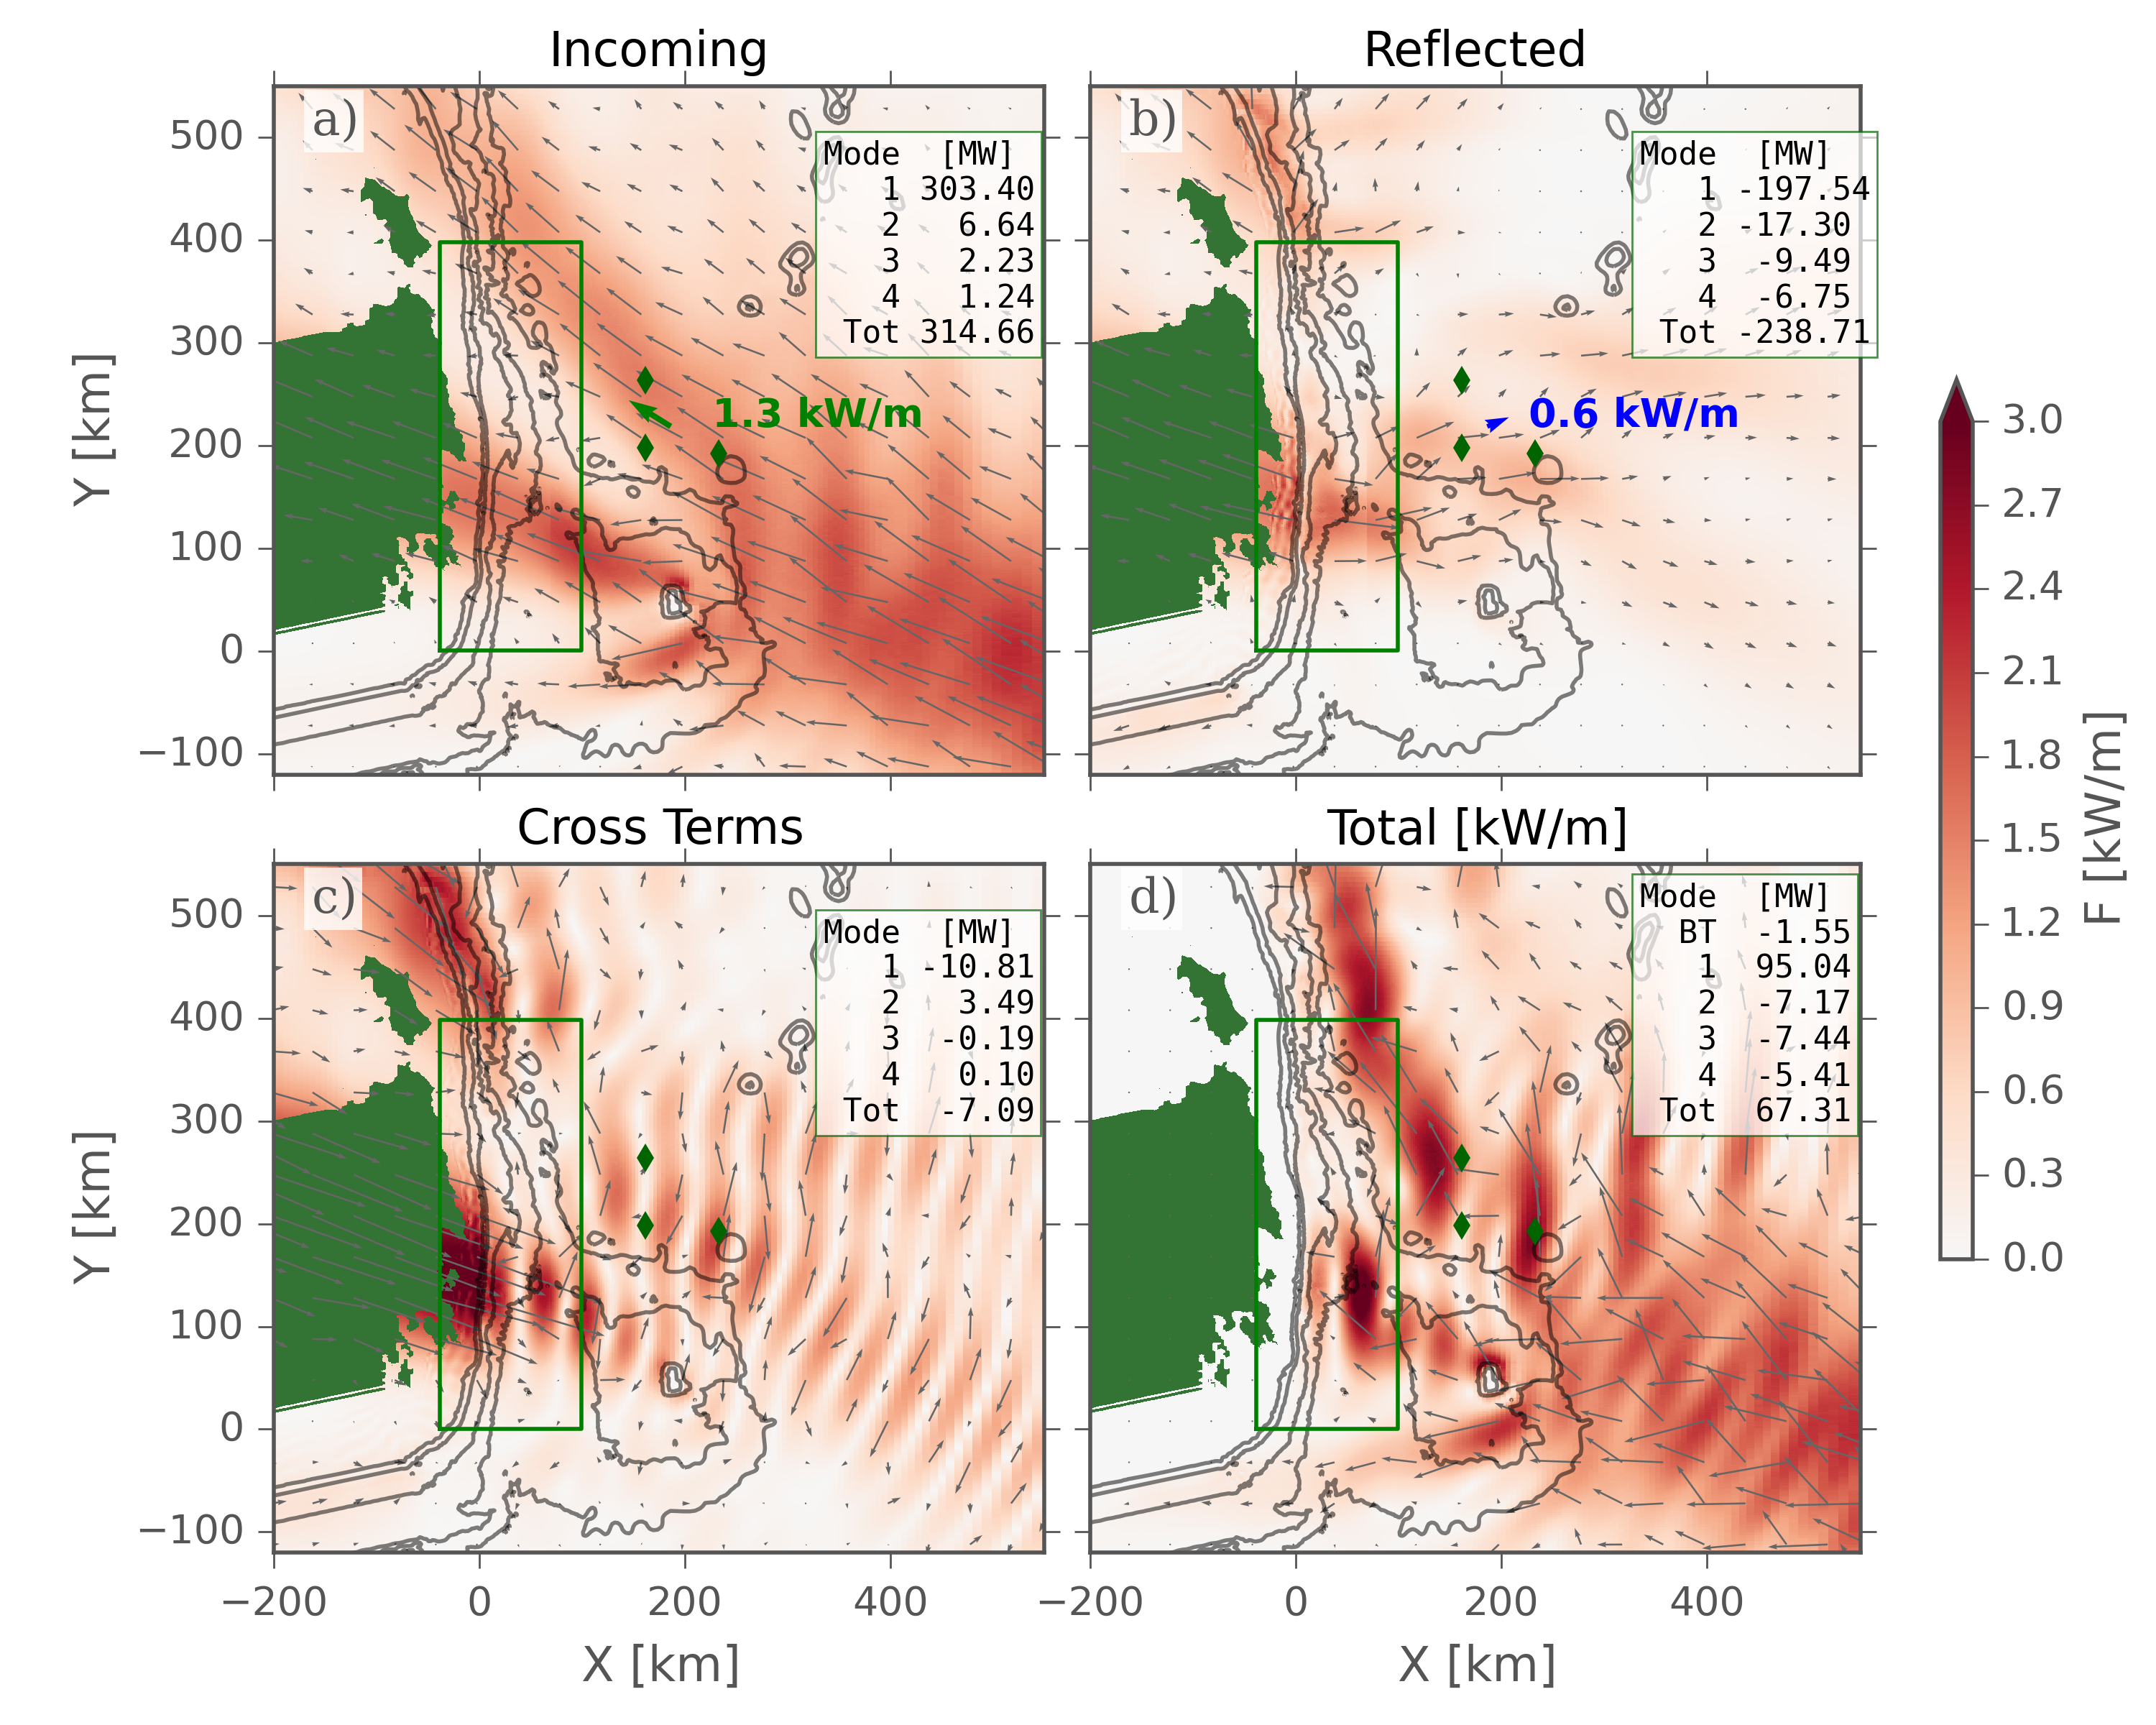
\includegraphics[width=5.5in]{RealResponseMode1}
    \caption{Energy partition as in \fref{fig:ShelfResponseMode1}, taking the \mn{Rise} simulation as the incoming wave, and \mn{Real} simulation as the total wavefield.  
      \tempS{\footnotesize /Users/jklymak/ttide/ProcessHaiseTas3d.ipynb ;     
        /Users/jklymak/ttide/doc/RealResponseMode.pdf}
      } \label{fig:RealResponseMode1}
  \end{center}
\end{figure*}

\section{Discussion}
\label{sec:Discussion}
\subsection{Estimating reflection co-efficients}

A major goal of this effort is estimating the fraction of incoming tide that is reflected by the Tasman continental slope to come up with a reflectivity co-efficient. Here we discriminate between the mode-1 reflection, $R_1=F_{ref,1}/F_{in,1}$, and the total reflection into all the modes, $R_T=F_{ref}/F_{in}$. Evaluating these co-efficients is less straightforward than it may sound because it is difficult to separate the incoming from reflected signal in complicated geometry, even in a fully resolved numerical model, let alone in observations.  Above, we used an integrated measure, comparing the incoming flux from a model with no continental slope to one with a continental slope and integrating the fluxes over a control volume from $y=$0 to 400 km.  This control volume was an arbitrary choice, but yielded reflectivities of mode -1 internal tide $R_1=0.65$ and the total internal tide of $R_T=0.76$ (\fref{fig:RealResponseMode1}). 

Determining reflectivity from a mooring array is significantly complicated by three-dimensionality and along slope variability.  From the mooring array in \fref{fig:RealResponseMode1}, the reflectivity is $R_1=0.6/1.3=0.46$, a significant under-estimate.  The reason for this should be relatively clear from looking at \fref{fig:RealResponseMode1}a,b; the mooring array nicely captures the northward diffracted ray, but catches some of the reflected pattern from the main beam to the south. There are significant interferences in the reflected patterns (\fref{fig:RealResponseMode1}b) because the reflected pattern is a complicated superposition of the cylindrically spreading reflections along the slope.  

Determining the reflectivity as a function of along-slope direction $y$ is difficult.  Simply lining up the onslope fluxes does not yield useful results because the reflection from any given point on the slope radiates cylindrically, and it is necessary to integrate over volumes.  Here we take the same approach as used in the previous section (i.e. \fref{fig:RealResponseMode1}), but integrate over smaller control volumes (80 km in $y$) to see the reflectivity as a function of $y$ (\fref{fig:TwoDReflectivity}a,b).  The incoming flux every 80 km shows the diffracted beam pattern with a maximum net incoming flux at $y=120\ \mathrm{km}$ (\fref{fig:TwoDReflectivity}a, red line) and a secondary peak to the north at about $440\ \mathrm{km}$.  The net reflectivity from these boxes ranges from 0.8 to a low of almost zero at $y=280\ \mathrm{km}$ (\fref{fig:TwoDReflectivity}b, solid blue line).  Note an uncertainty in the flux decomposition associated with the flux in the cross terms (\fref{fig:TwoDReflectivity}a, purple line).  This term does not balance to zero, and forms a significant part of the energy budget over such small control volumes.  It cannot be uniquely decomposed into either the incoming or reflected energy terms, so remains as an uncertainty. 

\begin{figure*}[htbp]
  \begin{center}
    \includegraphics[width=\twowidth]{TwoDReflectivity}
    \caption{a) Energy budget from 80 km by 80 km control volumes along the continental slope from the \mn{Real} simulations.  The incoming flux (red) is compared to the reflected (blue) and the cross terms (purple).  b) The reflection co-efficients.  The blue line is $R_1$, the mode-1 reflectivity in the 80-km control volumes along slope from the non-linear simulation.  The black line is the mode-1 reflectivity from a linear model \citep{kellyetal13b}, and the grey lines behind are the cumulative sum of modes 2, to 5 and then all the modes.  These do not sum up to one because the linear model has some ``viscosity'' that removes some high-mode energy.  The dashed lines are the mean of $R_1$ from the linear model if a constant average is taken (light blue, dashed), and if weighted by the diffracted beam strength (purple, dashed).  
      \tempS{\footnotesize /Users/jklymak/ttide/CELT/doc//CELTModel.ipynb ;     
        /Users/jklymak/ttide/CELT/doc/TwoDReflectivity.pdf}
      \label{fig:TwoDReflectivity} }
  \end{center}
\end{figure*}

In two-dimensions, the fraction of the tide reflected into mode 1 (and higher) can be predicted from linear theory using the method described by \citet{kellyetal13b} of matching Laplacian tidal solutions at discrete steps on a discretized topography.   If the tide is obliquely incident on the slope, there can be substantial differences in the reflected tide \citep{kellyetal13a}.   If we run these solutions for the Tasman Slope with an incident angle of 30 degrees, the reflectivity into mode-1, $R_1$ is similar to the numerical simulation (\fref{fig:TwoDReflectivity}b, thick black line).  The predicted reflectivity is greater for most of the ridge, but the null at $y=250\ \mathrm{km}$ is captured.  

The \mn{Real} simulation has a mode-1 reflectivity of $R_1=0.65$. A naive average of the reflectivity from the linear model between $y=0$ and $400\ \mathrm{km}$ yields $\left<R_1\right> = 0.71$.  However, that does not take into account the varying strength of the incoming diffracted beam, which is stronger where the reflectivity is higher.  Weighting by the incoming beam strength, then the reflectivity averages $\left<R_1\right>_{beam}=0.8$, and is substantially larger than in the numerical simulations.  

An attempt has been made to estimate reflectivity from this site from autonomous gliders surveys \citep{johnstonetal15}.  First, the gliders saw a substantial concentration of energy shoreward of the Tasman Rise.  This is a feature of the model, and clearly explained by the diffraction of energy by the Tasman Rise (\fref{fig:RealResponseMode1}).   

For the region in the lee of the Tasman Rise, \citet{johnstonetal15} estimate a reflectivity of the mode-1 internal tide of between 0.8 to 1.0 by fitting plane waves to the velocity and displacement amplitudes and phases.  If we confine our incoming versus outgoing energy budget to the region $80\ \mathrm{km}< y < 200\ \mathrm{km}$, representative of their \emph{Spray 56} deployment, we calculate a reflectivity of 0.7, which is lower than their lowest estimate of 0.8, and much lower than their high estimate of 1.0.  A second deployment, \emph{Spray 55}, covered more of the slope (up to $y=300\ \mathrm{km}$).  In this domain, they estimate a reflectivity of 0.6.  This is in agreement with the numerical simulation, which achieves  the same result from $0\ \mathrm{km}< y < 300\ \mathrm{km}$.  

The directions of wave propagation fit from the glider data is not in agreement with the model.  The fits to the \emph{Spray 55} data show incoming energy at between 125 and 145 degrees, which is similar to the model.  However the reflection is slightly south of due east (0 to -30 degrees geographic), whereas the numerical model is definitely to the northeast far from shore.  An explanation is evident from close inspection of \fref{fig:RealResponseMode1}b between the Tasman Rise and the continental slope where the glider spent the most time.  At this location the off-shore energy flux is almost exactly in the x-direction, (-12 degrees geographic), in agreement with the glider observations.  

Finally, one of the gliders (\emph{Spray 56}) picked out a northward propagating disturbance along the continental slope with wavelength of 100 km.  This wavelength matches the wavelength of the slope wave seen in the real simulations (\fref{fig:DissReal1km03}a,b).  Interestingly, they only pick this wavelength out in vertical displacement data, not in velocity.  


\subsection{Slope wave importance and dynamics}

\begin{figure*}[htbp]
  \begin{center}
    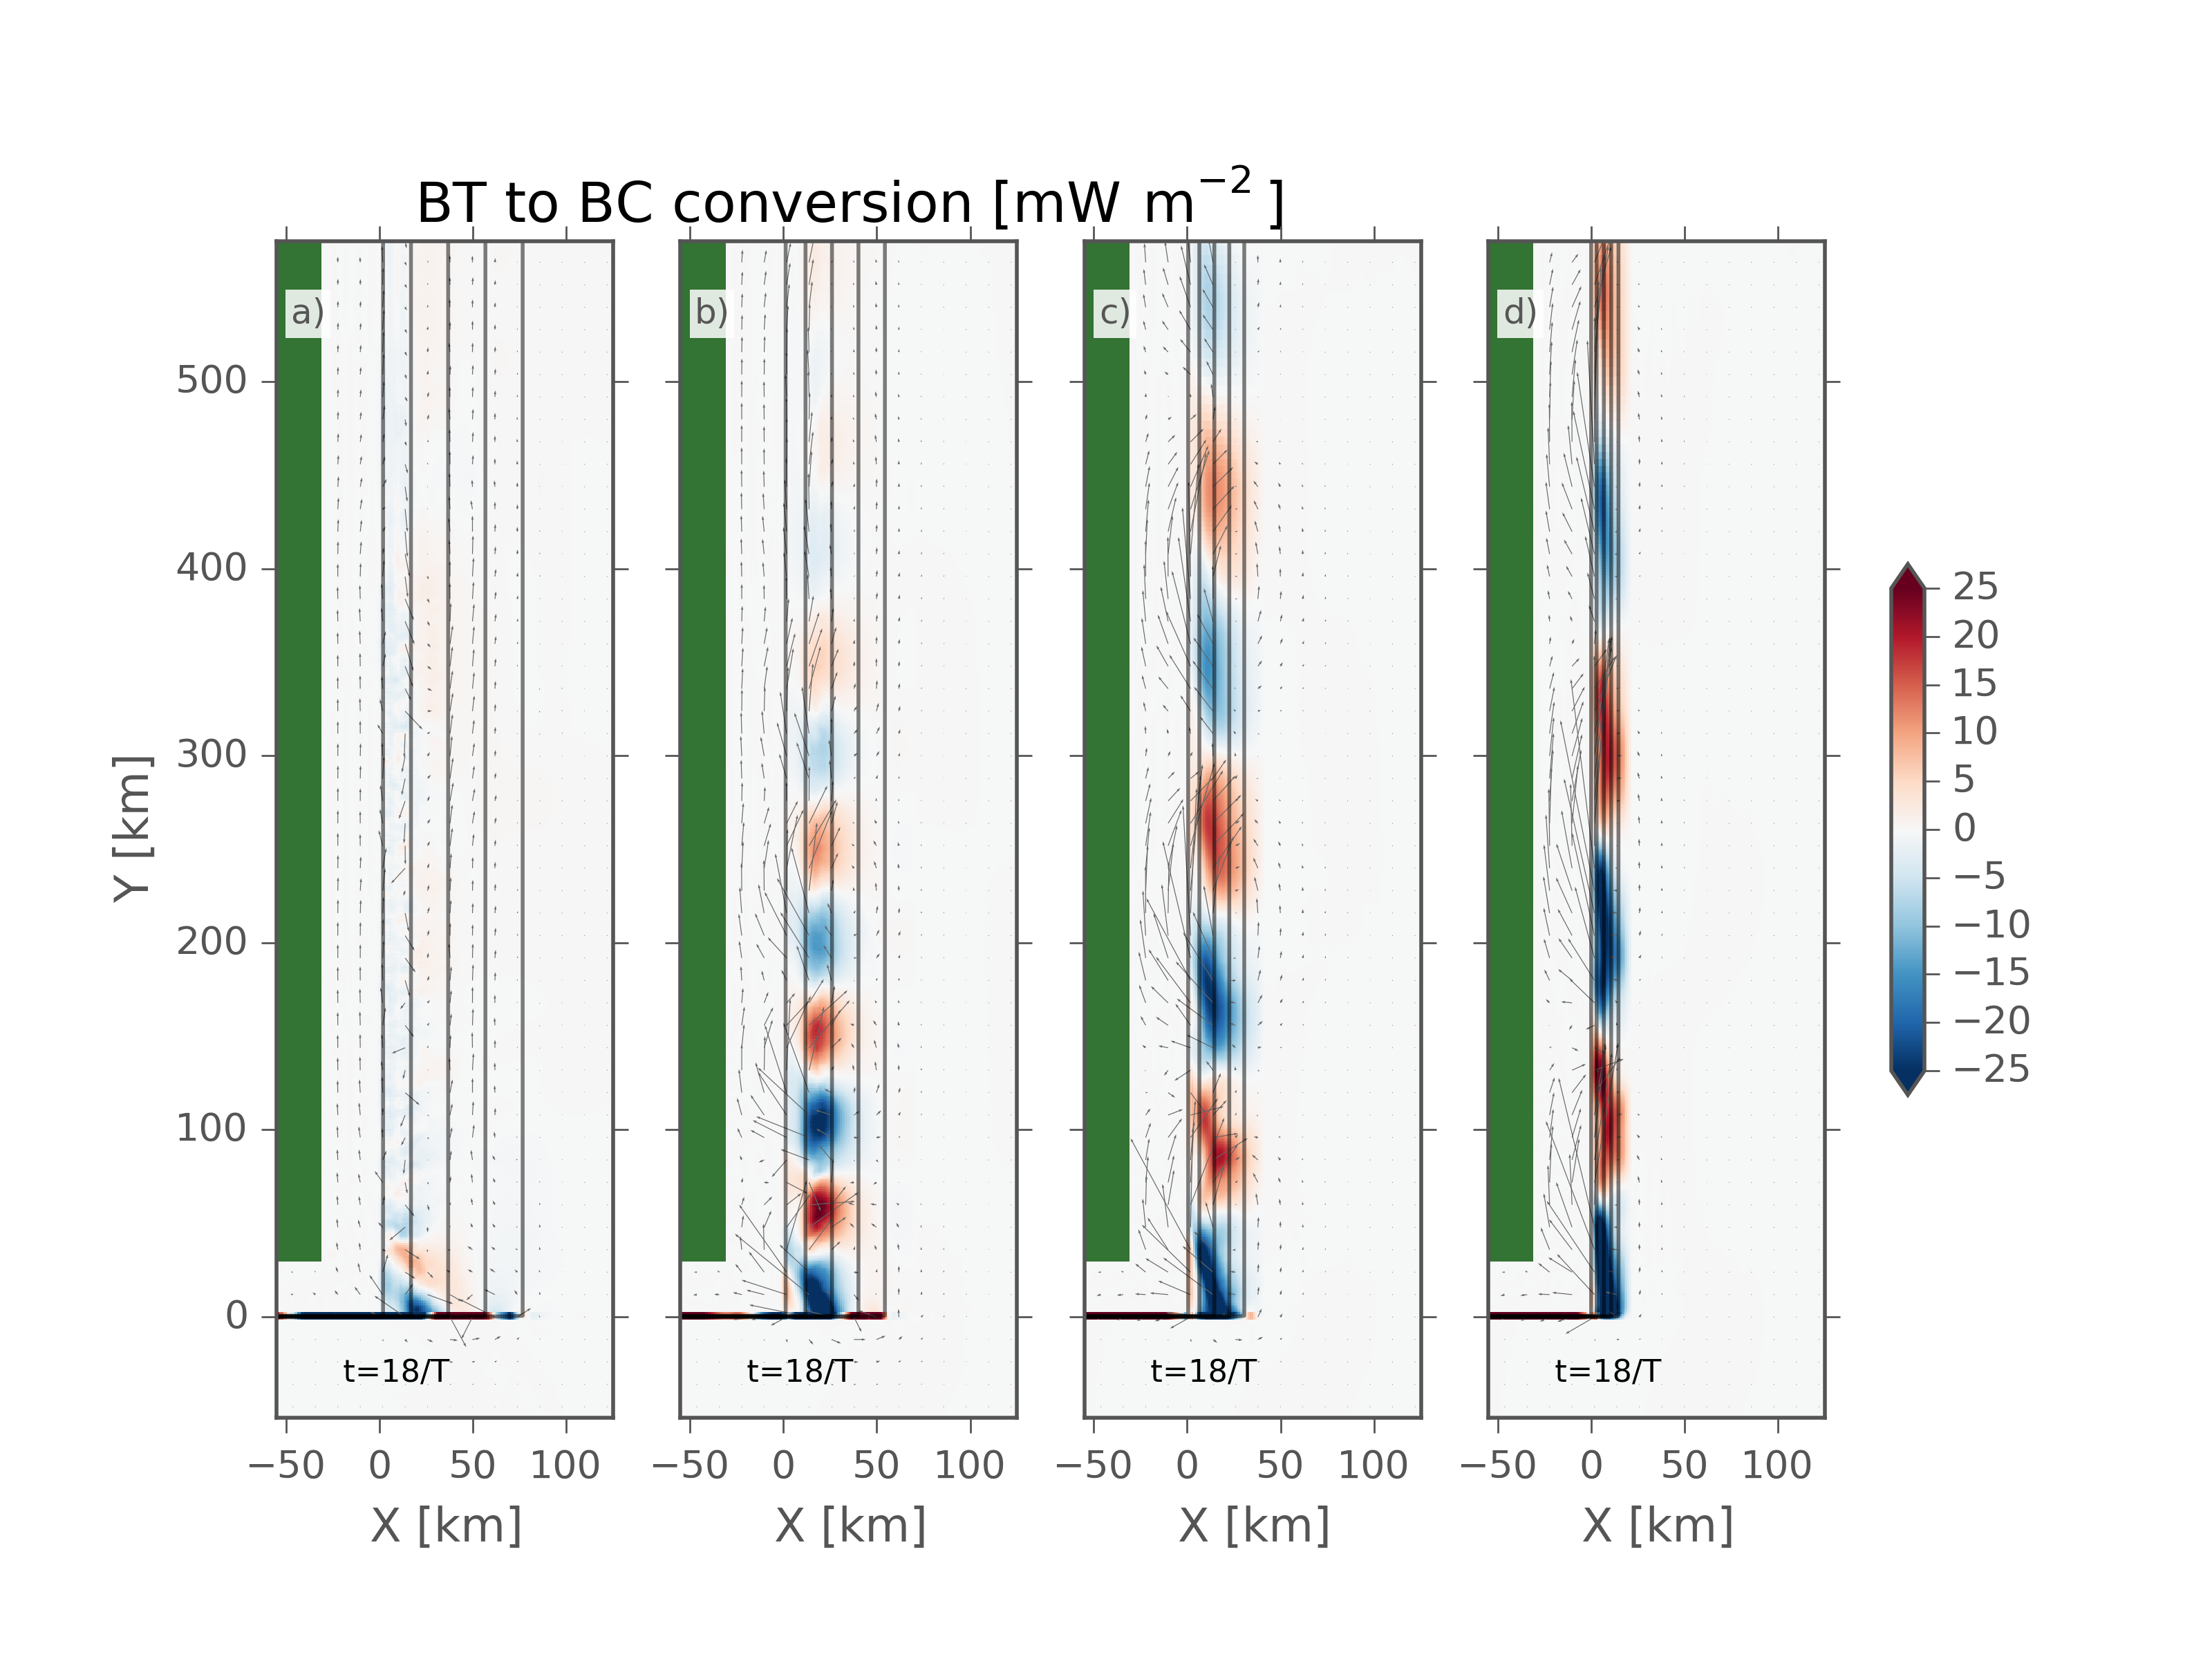
\includegraphics[width=6in]{ShelfWidthBTBC}
    \caption{Barotropic to baroclinic conversion for different shelf widths from widest (a) to narrowest (d).  Arrows are barotropic flux vectors.  Note how the along-slope barotropic flux is almost entirely confined to conversion dipoles along slope.
      \tempS{\footnotesize /Users/jklymak/ttide/ttide15/doc//PaperPlots.ipynb ;     
        /Users/jklymak/ttide/ttide15/doc/ShelfWidthBTBC.pdf}
       }\label{fig:ShelfWidthBTBC}
  \end{center}
\end{figure*}

%\begin{figure}[htbp]
%  \begin{center}
%    \includegraphics[width=3in]{BarotropicResponseShelf1km04}
%    \caption{Barotropic response for the \mn{Shelf} case.  
%      \tempS{\footnotesize /Users/jklymak/ttide/ProcessHaiseTas3d.ipynb ;     
%        /Users/jklymak/ttide/doc/BarotropicResponseShelf1km04.pdf}
%      \label{fig:BarotropicResponseShelf1km04} }
%  \end{center}
%\end{figure}

The structure of the barotropic-to-baroclinic conversion on the slope is an intriguing feature of these simulations, and appears in regional simulations (Simmons, in prep) and the glider data \citep{johnstonetal15}.  Here, it shows up most clearly in the \mn{Shelf} simulations because of the simplified bathymetry.  However, it is also clear in the \mn{Real} simulation (\fref{fig:DissReal1km03}a).  This slope wave redistributes energy in the reflected baroclinic response (\fref{fig:ShelfResponseMode1}), taking a relatively homogenous incoming energy source and focusing the reflection every 200 km or so along slope.

This wave is a slope mode that is strummed by the incident internal tide at the ``corner'' of the topography ($x=0$, $y=0$);  a long slope without the corner does not excite this wave, nor does an internal tide coming directly from the east and hitting the topography at a normal angle.  The along-slope wavelength is independent of the incident along-slope wavelength in the open water (tested by changing the angle of the incident tide; not shown), and is a robust feature of the slope shape.   A sensitivity experiment that varied the continental slope widths demonstrates that narrower slopes strum longer along-slope waves (\fref{fig:ShelfWidthBTBC}).

These waves are super-inertial and are an example of partially trapped slope waves \citep{dalesherwin96,daleetal01}. We compare the wavelength of the slope waves (\fref{fig:AlongSlopeCompare}, thick lines) to the empirical modes predicted from linear theory \citep{daleetal01}.  The procedure solves for the response of the flow in the coastal bathymetry due to forcing with varying along-slope wavelengths.  Resonant along-slope wavelengths lead to a much stronger response (Appendix and \fref{fig:AlongSlopeCompare}, thin lines).  The along-slope wavelength of the resonant modes in the linear calculation agree quite well with the wavelengths of the fully non-linear solutions.  Narrower continental slopes yield longer along-slope wavelengths, and the spatial modes that correspond to the peaks are similar to deep-ocean mode-1 off the slope. 

\begin{figure*}[htbp]
  \begin{center}
    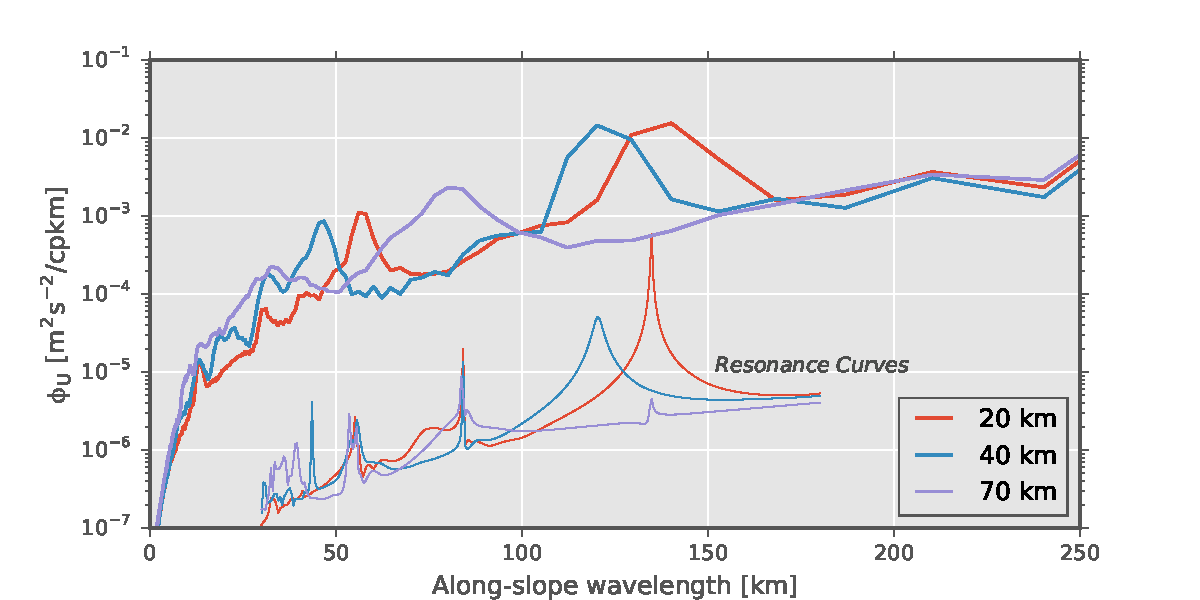
\includegraphics[width=6in]{AlongSlopeCompare}
    \caption{Along-slope spectra of across slope velocity (thick lines) for the three narrowest slopes in \fref{fig:ShelfWidthBTBC}, from velocities on the shallow shelf in these simulations.  The thin lines are resonance curves, formed from the cross-slope equations of motion assuming harmonic motion in time and along-slope.  As along-slope wavenumber is varied resonant modes have a stronger response.  What is plotted is arbitrary units for the three slope geometries.  
      \tempS{\footnotesize /Users/jklymak/ttide/ttide15/doc//PaperPlots.ipynb ;     
        /Users/jklymak/ttide/ttide15/doc/AlongSlopeCompare.pdf}
      \label{fig:AlongSlopeCompare} }
  \end{center}
\end{figure*}

The slope wave is an important term in the local energy budget  when compared the incoming and reflected energy fluxes (\fref{fig:ShelfEnergyInt}).  The incoming energy peaks at 1.2 kW/m, and the reflected energy is of a similar magnitude but with oscillations at twice the wavelength of the slope wave.   The integrated barotropic-baroclinic conversion is as high as 0.4 kW/m-coastline, and leads to 0.4 kW/m peak-to-peak oscillation in the reflected energy (its not 0.8 kW/m peak-to-peak because the reflected energy spreads spherically by 40 km, where the reflected flux is evaluated, \fref{fig:ShelfResponseMode1}).  This turns even a relatively straight slope into a series of internal tide absorbers and radiators, leading to 100-km scale inhomogeneity in the reflected internal tide.  

\begin{figure}[htbp]
  \begin{center}
    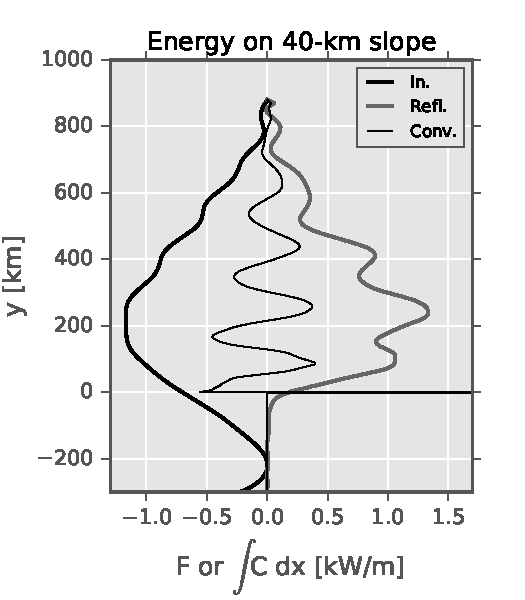
\includegraphics[width=2.5in]{ShelfEnergyInt}
    \caption{Terms from the energy budget for 40-km wide slope.  The incoming and reflected energy fluxes are computed at $x=40\ \mathrm{km}$, and the conversion term integrated from the shelf to $x=40\ \mathrm{km}$.  
      \tempS{\footnotesize /Users/jklymak/ttide/ttide15/doc//PaperPlots.ipynb ;     
        /Users/jklymak/ttide/ttide15/doc/ShelfEnergyInt.pdf}
      \label{fig:ShelfEnergyInt} }
  \end{center}
\end{figure}

\section{Summary}
\label{sec:Summary}

A mode-1 internal tide was launched at a variety of topographies representing the Tasmanian continental slope.  The goal was to determine the ``reflectivity'' of this slope, in terms of the modal content of the reflected energy and the local dissipation.  The latter is somewhat suspect in this model because of crude lateral resolution, but the \mn{Real} simulation indicated that 21\% of the incoming energy was dissipated, and 65\% was reflected as mode-1 energy.  The incoming internal tide flux used here was  weak compared to the flux modeled and inferred from altimetry in the Tasman Sea, so we expect the dissipation in more realistically forced models to increase.  

Despite a simple incoming internal tide that is linear, semi-diurnal, and mode-1, we have found a rich and complex response of the topography when the remote wave impacts the topography.  The response can be characterized as follows:
\begin{itemize}
  \item diffraction of the beam by the Tasman Rise,
  \item oblique reflection from the continental slope,
  \item and a leaky slope wave response that redistributes reflected internal energy along-slope.  
\end{itemize}
Of these, perhaps only the second effect was expected before carrying out the simulations.  However, as we saw above, even the reflection problem is significantly complicated in the presence of three-dimensionality.  

Diffraction around underwater topography should have been expected, however, the relative depth of the obstacle makes it surprising that the effect is so strong.  The fact that the lateral width  of the Tasman Rise is close to the wavelength of the incoming internal tide makes predicting the diffraction pattern difficult.  \citet{baines07} considers generation of internal tides at seamounts, but does not deal with scattering and diffraction.  The problem is similar to electromagnetic waves passing through a wire, but a linear response for that problem is not trivial to compute \citep[i.e.][]{bonod2005differential}, and still does not have a confined vertical mode structure as we find in the internal wave problem.

The excitation of slope waves has been explored by \citet{daleetal01}. It has an important effect on the redistribution of energy along slope.  The redistribution affects where high dissipation is found in the model (\fref{fig:DissReal1km03}), and adds more inhomogeneity to the reflected internal tide.    

The complexity grows if other real-world influences are to be accounted for.  The East Australian Current flows along this slope, varying the stratification in the horizontal, provides lateral shears that can distort the internal tide response, and carrying eddies that can add a strong time dependence to these effects.  Even in two dimensions, the strength of the  internal tide reflection can be significantly impacted by the phase of the incoming tide with other baroclinic modes \citet{klymaketal11a} or the barotropic \citep{kellynash10}.
The simulations here exclude the local barotropic tide, so this would certainly complicate the reflected response.  Finally, the internal tide used here was monotonic, whereas the real tide will also have other frequencies, most notably subinertial diurnal frequencies that will have trapped wave responses (personal communication, R. Musgrave).  

Regardless, it is useful to have studied the ``simplest'' response we could in this system to tease apart the dominant physics.  This response is complex, and it should be clear that solely observational efforts to balance a reflection budget are going to be a challenge.  Merging simulations and observations is a likely way forward in understanding the wave field in this complex slope region.

With respect to the reflection problem, the modeled slope has a relatively high reflection back into the open ocean, with as much as 65\% of the incoming energy being reflected as mode-1.  Its possible that higher resolution runs will be more dissipative, and that stronger forcing will lead to a higher fraction of dissipation.  However, these simulations, and the results from the rest of the experiment to date \citep[i.e.][]{johnstonetal15} indicate that bulk of the energy from the Macquarie Ridge must dissipate elsewhere.  

\begin{acknowledgment} 
Our thanks to conversations with Andy Dale on leaky slope waves and Qiang Li for sharing his linear code for the Lindzen-Kuo method.  
J. Klymak was supported by the Canadian National Science Engineering Research Council Discovery Grant 327920-2006, and by computer time from the US Office of Naval Research, T. Paluszkiewicz, program officer.  H. Simmons and D. Brazhnikov were supported by NSF OCE 1130048.  J.\ MacKinnon, and R.\ Pinkel were supported by award  NSF OCE 1129763. M.\ Alford was supported by NSF OCE 1129246.
 A website for this paper with analysis scripts, intermediate data files, and model setups is at \url{http://web.uvic.ca/~jklymak/ttide15}.  

\end{acknowledgment}

% Use appendix}[A], {appendix}[B], etc. etc. in place of appendix if you have multiple appendixes.
\ifthenelse{\boolean{dc}}
{}
{\clearpage}
\begin{appendix}

\section*{\begin{center}Appendix Slope-wave calculation\end{center}}

The slope wave calculation follows the calculation made by \citet{daleetal01}, where there are more details.  The linear equation for the pressure perturbations are assumed to have form $P = p(x,z) \exp^{i(k_y y - \omega t)}$, where $k_y$ is the along-slope wavenumber. 
\begin{equation}
  \left(f^2 - \omega^2\right)\frac{\partial}{\partial z} \left( \frac{\partial p/\partial z}{N^2-\omega^2}\right) + \frac{\partial^2 p}{\partial x^2} - k_y^2 p = 0
\end{equation}
Subject to boundary conditions at the surface of $\partial p / \partial z = 0$ and at the sea floor of 
\begin{equation}
  \left( \frac{\omega^2-f^2}{N^2-\omega^2} \right)\frac{\partial p}{\partial z } = \frac{\partial h}{\partial x}\left(\frac{\partial p}{\partial x} -\frac{fk_y}{\omega} p \right)  
\end{equation}
The coast is assumed to be a wall, and the open ocean to consist of waves radiating away from the slope, or if $k_x$, the cross-slope wavenumber, is imaginary, disturbances that decay away from the slope.  

The above are discretized on a domain that is 260 km wide into 261 grid cells in $x$, and onto a sigma-co-ordinate with 192 vertical levels.  The hyperbolic method of solution due to \citet{lindzenkuo69} was used to solve on this domain for $p$ for $\omega = 1.4 f$, $f = 10^{-4} \mathrm{s^{-1}}$, and for a sweep of $k_y$.  Under an arbitrary forcing certain values of $k_y$ resonate and lead to stronger amplitude responses in $p$ corresponding to spatial modes of the system.  The numerical method is sensitive to the stratification, so we used a fit exponential of $N^2(z) = 2\times10^{-5}\mathrm{s^{-2}}\ e^{z/(1000\ \mathrm{m})}$ (where $z$ is negative downwards).  The scan was taken over 300 wavelengths equally spaced between $30$ and $180\ \mathrm{km}$.  

The resulting spatial modes are similar to those in \citet{daleetal01} (\fref{fig:FitModes}).  There is a peak of amplitude on the shelf, and then a second peak on the slope.  As the slope gets more narrow, the peak on the slope becomes broader.  These shapes are the lowest modes.

\begin{figure*}[htbp]
  \begin{center}
    \includegraphics[width=6in]{FitModes}
    \caption{Spatial shape of modes picked out from the resonant searching technique (as shown in \fref{fig:AlongSlopeCompare}) for the 70, 40 and 20-km wide slopes.  
            \label{fig:FitModes} }
  \end{center}
\end{figure*}

The general code to solve this is at \url{https://github.com/jklymak/LindzenKuo}.  The exact code used for this paper is with the rest of the supplemental material.  

%\subsection{First appendix secondary heading}
%
%\subsection{Second appendix secondary heading}
%
%\subsubsection{First appendix tertiary heading}
%
%\subsubsection{Second appendix tertiary heading}
%
%\paragraph{First appendix quaternary heading}
%
%\paragraph{Second appendix quaternary heading}
%
\end{appendix}

% Create a bibliography directory and place your .bib file there.
% -REMOVE ALL DIRECTORY PATHS TO REFERENCE FILES BEFORE SUBMITTING TO THE AMS FOR PEER REVIEW
\ifthenelse{\boolean{dc}}
{}
{\clearpage}
\bibliographystyle{ametsoc}
\bibliography{main}

%%%%%%%%%%%%%%%%%%%%%%%%%%%%%%%%%%%%%%%%%%%%%%%%%%%%%%%%%%%%%%%%%%%%%
% FIGURES-REMOVE ALL DIRECTORY PATHS TO FIGURE FILES BEFORE SUBMITTING TO THE AMS FOR PEER REVIEW
%%%%%%%%%%%%%%%%%%%%%%%%%%%%%%%%%%%%%%%%%%%%%%%%%%%%%%%%%%%%%%%%%%%%%

%
\end{document}